\chapter
 [NetQASM: A low-level instruction set architecture for hybrid quantum-classical programs in a quantum internet]
 {NetQASM: A low-level instruction set architecture for hybrid quantum-classical programs in a quantum internet}
\label{chp:netqasm}


\begin{abstract}
    We introduce NetQASM, a low-level instruction set architecture for quantum
    internet applications. NetQASM is a universal, platform-independent and
    extendable instruction set with support for local quantum gates, powerful
    classical logic and quantum networking operations for remote entanglement
    generation. Furthermore, NetQASM allows for close integration of classical
    logic and communication at the application layer with quantum operations at
    the physical layer. This enables quantum network applications to be
    programmed in high-level platform-independent software, which is not
    possible using any other QASM variants. We implement NetQASM in a series of
    tools to write, parse, encode and run NetQASM code, which are available
    online. Our tools include a higher-level SDK in Python, which allows an easy
    way of programming applications for a quantum internet. Our SDK can be used
    at home by making use of our existing quantum simulators, NetSquid and
    SimulaQron, and will also provide a public interface to hardware released on
    a future iteration of Quantum Network Explorer.
\end{abstract}

\blfootnote{
This chapter is based on the publication:
\fullcite{dahlberg_2022_netqasm_noprint}.

A. Dahlberg and \textbf{B. van der Vecht} contributed equally to this work.
}

\iffullchapters
\section{Introduction}
\label{netqasm:sec:introduction}

\dropcap{Q}uantum mechanics shows
that if one is able to communicate quantum information between nodes in a
network, one is able to achieve certain tasks which are impossible using only
classical communication. There are many applications~\cite{Wehner2018stages}
where a \emph{quantum network} has advantage over a \emph{classical
      (non-quantum) network}, either by (1) enabling something that is theoretically
impossible in a classical network, such as the establishment of an
unconditionally secure key~\cite{bb84} and secure blind quantum
computing~\cite{childs2005assisted} or (2) allowing something to be done faster
or more efficiently such as exponential savings in
communication~\cite{Buhrman2010} and extending the baseline of
telescopes~\cite{gottesman2012longer}. In recent years, many experiments have
been conducted to show that a quantum network is not only a theoretical concept,
and indeed advancements have been made to implement such a quantum network on
various hardware platforms. \cite{Hensen2015, Humphreys2018,
      moehring2007entanglement, hofmann2012heralded, Kalb2017, Inlek2017,
      sangouard2011quantum}. However, these experiments alone do not yet make a
quantum network \textit{programmable}, since the program logic was hard-coded
into the experimental hardware ahead of time. (There have been examples of
      experiments with some simple logic but only with a very limited number of
      pre-loaded decision-branches.)

% Before considering how to program quantum network applications, let us first
% briefly sketch the system our applications are run on. Abstractly, quantum
% networks consist of \textit{nodes} that are connected by \textit{channels}
% (\cref{fig:network_model}). Classical channels enable classical communication
% between nodes, while quantum channels are used for \textit{entanglement}
% generation between nodes. So-called \textit{end-nodes} may contain
% \textit{quantum processors} that can run arbitrary (quantum) programs. They have
% access to a quantum memory consisting of qubits, on which they can perform
% operations, including quantum computations. Some of these qubits may be used for
% establishing an entangled quantum state with a remote node. An end-node also
% possesses a classical processor and a classical memory. Furthermore, an end-node
% can send and receive classical messages to and from other end-nodes in the
% network. A network of quantum networks may be a called a \textit{quantum
%       internet}.

% Quantum (network) processors differ from classical processors in a number of
% ways. Firstly, quantum memory has limited lifetime, meaning that its quality
% degrades over time. For example, quantum memories based on nitrogen-vacancy (NV)
% centers in diamond have impressively been optimized to achieve lifetimes in the
% order of seconds~\cite{Abobeih2018}; however, this is still very short compared
% to classical memories, which generally do not have a limited lifetime at all.
% Therefore, the quality of program execution is time-sensitive. Secondly,
% physical devices are prone to inaccuracies which lead to decreased quality of
% (quantum) computation. For example, applying an operation (like a gate) on a
% qubit affects that qubit's quality. We note that the two challenges mentioned so
% far are also inherent to non-network quantum processors. Quantum
% \textit{network} processors have additional challenges: (1) the processor may
% have to act as a local computation unit and a network interface at the same
% time; for example, in NV centers, an electron spin qubit is used for generating
% entanglement with a remote node but is also needed to do local two-qubit gates,
% (2) remote-entanglement operations may not have a fixed time in which they
% complete, which makes scheduling and optimization more difficult.

% Quantum network \textit{applications}, also called \textit{protocols}, are
% multi-partite programs that involve entanglement generation and classical
% communication between different end-nodes, as well as local computation.
% Examples include Quantum Key Distribution (QKD)~\cite{bb84, ekert1991quantum},
% leader election protocols~\cite{kobayashi2014simpler, ganz2009quantum}, and
% Blind Quantum Computation (BQC)~\cite{Wehner2018stages}. Such applications are
% split into distinct \textit{programs} each of which runs on a separate end-node.
% The programs consist of both local operations (classical and quantum) and
% network operations (classical and quantum), see \cref{fig:app_programs}. That
% is, the programs communicate either by passing classical messages, or by
% establishing quantum entanglement. For example, BQC involves a \textit{client}
% node and a \textit{server} node, both of which run their own program. Their
% joint execution looks roughly as follows: (1) The client and server engage in
% remote entanglement generation such that the server's quantum memory ends up
% being in a certain state, (2) the client sends instructions to the server in the
% form of a classical message, (3) the server performs a measurement-based
% computation on its own quantum memory based on the client's instructions, (4)
% the server sends measurement results back to the client, (5) the client sends
% new instructions based on the measurement results, (6) repeat steps 3 to 5 until
% the client obtains its desired result.

% The example above illustrates that quantum network programs consist of different
% types of operations. Indeed, program code consists of \textit{classical code},
% containing local classical operations and classical communication with other
% nodes, and \textit{quantum code}, which are operations on quantum memory (such
% as \textit{gates}) and remote entanglement generation. Blocks of these types of
% code may depend on each other in multiple ways, as depicted
% in~\cref{fig:program_decomp}. Programs with mixed classical and quantum
% operations have also been called \textit{dynamic quantum
%       circuits}~\cite{cross2021openqasm, burgholzer2021towards}, but these do not
% cover the networking dimension found in programs we consider here, such as the
% dependency on remote information and entanglement generation operations.

% Due to the nature of quantum network programs, execution may have to
% \textit{wait} for some time. For example, the program needs to wait until
% another node sends a classical message, or until remote entanglement has been
% established. Therefore, it makes sense to run multiple (independent) quantum
% network programs on a node at the same time (interleaved), so that processor
% idle times can be filled by execution of other programs. This is something that
% typically does not happen on local quantum computers, and therefore introduces
% new challenges.

% Quantum network applications may be programmed by a single actor. For example, a
% developer may program a QKD application in the form of a two programs, and
% distribute these two programs to two end-nodes in the network. Alternatively, a
% single-node quantum network program may be developed separately from other
% programs, possibly not knowing how these other programs are implemented. For
% example, a BQC service provider could have already implemented the server-side
% program of a specific BQC protocol. A client may then write the client-side of
% this protocol, without having control over the server-side implementation.

The aim of this work is to propose a way to program quantum network programs
and execute them on the end-nodes of a quantum network.


\begin{figure}[t]
    \centering
    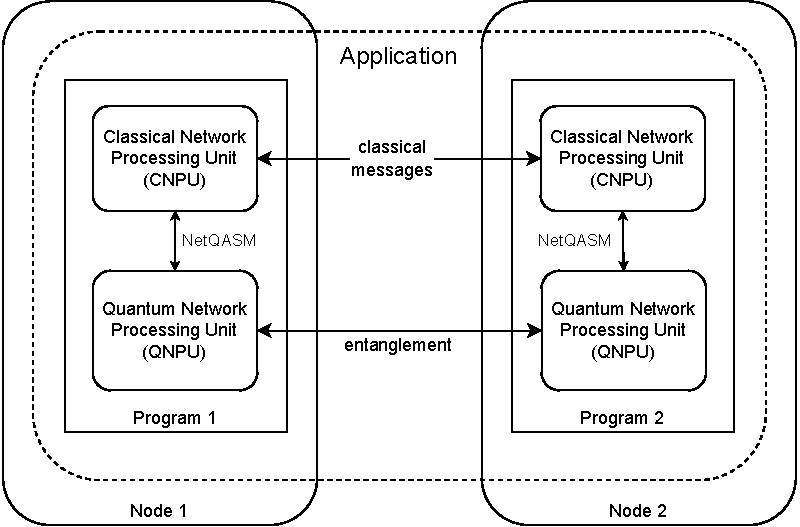
\includegraphics[width=0.6\linewidth]{figures/netqasm/multi_program_app_2.pdf}
    \caption{A quantum network application consists of a program for each of the nodes involved in the application.
        Each program is locally executed by the node.
        Program execution on each node is split into execution in an application layer, which can send and receive classical messages, and a quantum processor, which can create entanglement with another node.
        The communication between nodes can hence be both classical and quantum.
        Communication instructions need to be matched by corresponding instructions in the other program.
        There is no global actor overseeing execution of each of the programs, and the nodes may be physically far apart.}
    \label{fig:app_programs}
\end{figure}

\begin{figure}[t]
    \centering
    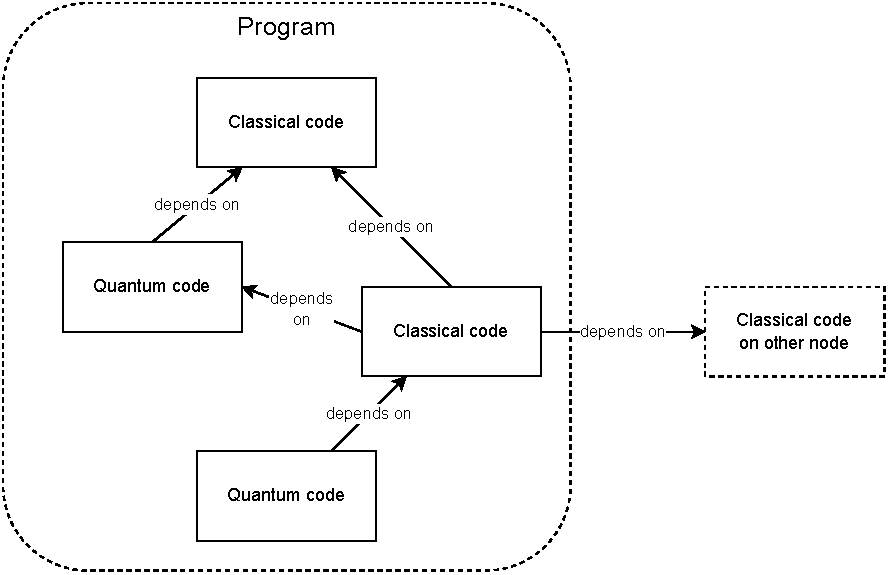
\includegraphics[width=0.6\linewidth]{figures/netqasm/program_decomp.pdf}
    \caption{A program on a single node consists of different blocks of code, which can be quantum (pure quantum instructions with classical control in between), or classical (no quantum operations at all).
        These blocks may depend on each other in various ways.
        For example, the outcome of a measurement happening in one of the quantum blocks may be used in a calculation performed in one of the classical blocks.
        Blocks may also depend on other nodes.
        For instance, the value of a message coming from another node can influence the branch taken in one of the classical blocks.}
    \label{fig:program_decomp}
\end{figure}


In this chapter we introduce an abstract model---including a \ac{QNPU}--- for end-nodes in a quantum network, which we define in~\cref{netqasm:sec:preliminaries}.
We then propose \ac{NetQASM}, an instruction set architecture that can be used to run arbitrary programs (of the form described in \cref{fig:program_decomp}) on end-nodes, as long as the end-nodes realize the model including the QNPU.

\ac{NetQASM} consists of a specification of a low-level assembly-like language to express the quantum parts of quantum network program code.
It also specifies how the application layer should interact with the \ac{QNPU} and how the assembly language can be used to execute (network) quantum code.
This is not possible using other QASM languages.

The \ac{NetQASM} language is extendible using the concept of \textit{flavors}.
The core language definition consists of a common set of instructions that are shared by all flavors.
This common set contains classical instructions for control-flow and classical memory operations.
This allows the realization of low-level control logic close to the quantum hardware;
for example, to perform branching based on a measurement outcome.
Quantum-specific instructions are bundled in flavors.
We introduce a \textit{vanilla} flavor containing universal platform-independent quantum gates.
Using this flavor of the \ac{NetQASM} language enables the platform-independent description of quantum network programs.
Platform-\textit{specific} flavors may be created to have quantum operations that are native and optimized for a specific hardware platform.
As an example, we show a flavor tailored to the Nitrogen-Vacancy (NV) hardware, a promising platform for quantum network end-nodes~\cite{Taminiau2014, hanson2021realization}.

In our model, application-specific classical communication only happens at the application layer (\cref{fig:app_programs}).
In particular, this means that \ac{NetQASM} contains no provision for classical communication with the remote node.
We remark that of course, classical control communication may be used by the \ac{QNPU} to realize the services of the quantum network stack accessed through \ac{NetQASM}.

We note that \ac{NetQASM} is used for representing and running code that runs on a single node in a quantum network.
Synchronization between the (\ac{NetQASM}) programs of multiple nodes is the responsibility of the programmer.
For example, in a client-server application, if the client code contains a `receive classical message' operation, it is the responsibility of the server node that its program code contains a `send classical message' operation at the right moment.
The same holds for instructions for creating remote entanglement.
In terms of precise timing, which is needed for entanglement generation, it is the \ac{QNPU} that is responsible to communicate and synchronize with the \ac{QNPU} of the other node to make sure entanglement attempts are synchronized.

With \ac{NetQASM}, we solve various problems that are unique to quantum internet programming:
    (1) for remote entanglement generation, we introduce new instruction types for making use of an underlying quantum network stack~\cite{dahlberg2019linklayer, kozlowski2020networklayer},
    (2) for the close interaction between classical and quantum operations, we use a shared-memory model for sharing classical data between the application layer and the \ac{QNPU},
    (3) in order to run multiple applications on the same quantum node---which may be beneficial for overall resource usage (see~\cref{netqasm:sec:design_considerations})---we make use of virtualized quantum memory, similar to virtual memory in classical computing~\cite{arpaci2018operating},
    (4) since on some platforms, not all qubits may be used to generate remote entanglement, we introduce the concept of unit-modules describing qubit topologies with additional information per (virtual) qubit about which operations are possible.

Since \ac{NetQASM} is meant to be low-level, similar in nature to classical assembly languages, we have also developed a higher-level software development kit (SDK), in Python, to make it easier to write applications.
This SDK and related tools are open-source and freely available at~\cite{git_netqasm}, as part of our Quantum Network Explorer~\cite{qne_website}.
Through the SDK we have also enabled the quantum network simulators NetSquid~\cite{coopmans2021netsquid} and SimulaQron~\cite{dahlberg2018simulaqron} to run any application programmed in \ac{NetQASM}.

We have evaluated \ac{NetQASM} by simulating the execution of a teleportation application and a blind quantum computation using \ac{NetQASM}.
Hereby we have shown that interesting quantum internet applications can indeed be programmed using \ac{NetQASM}.
Furthermore, the evaluations argue certain design choices of \ac{NetQASM}, namely the use of so-called \textit{unit modules}, as well as platform-specific
\textit{flavors}.

We remark that \ac{NetQASM} has already been used on a real hardware setup in the lab, in a highly simplified test case that only produces entanglement~\cite{pompili2021experimental}.
\todo{refer to next chapter in which full stack has been implemented}


\subsection{Related Work}
\label{netqasm:sec:related}

\todo{Remove parts that are already in Background chapter and just refer to them}
In the field of quantum computing, a substantial amount of progress has been made related to developing
architectures (e.g.~\cite{fu2017microarchitecture,bourassa2020photonicblueprint, murali2019fullstack, wecker2014liqui, khammassi2020openql, amy2019staq, green2013quipper, Steiger2016}),
instruction sets (e.g.~\cite{cross2017openqasm,khammassi2018cqasm,fu2019eqasm,liu2017fqasm,smith2016quil,qiskit,cirq,qsharp,jones2019quest}) and
compilers~\cite{zulehner2019compiling, haner2018software, gokhale2020quantum, liu2020new, gokhale2020optimized, ding2020square, smith2020opensource, Sivarajah_2020, hietala2019verified, zhang2020contextmapping, niu2020hardware, dury2020qubo, pozzi2020using, Nishio_2020}.
One example is QASM, an instruction set framework, borrowing ideas from classical assembly languages, which has gained a lot of popularity over the years and has been successfully integrated in software stacks for quantum computers.
There are in fact many variants of QASM such as OpenQASM~\cite{cross2017openqasm}, \texttt{cQASM}~\cite{khammassi2018cqasm}, \texttt{eQASM}~\cite{fu2019eqasm}, \texttt{f-QASM}~\cite{liu2017fqasm}.
Some of these variants are at a level closer to the physical implementation, such as \texttt{eQASM}, allowing for specifying low-level timing of quantum operations, while others, such as \texttt{f-QASM}, are at a higher level.
Together with the definition of these QASM-variants, progress has also been made in compilation of applications programmed in QASM to hardware implementations.
More abstract languages and programming frameworks for quantum programs include \texttt{Quil}~\cite{smith2016quil}, \texttt{Qiskit}~\cite{qiskit}, \texttt{Cirq}~\cite{cirq}, \texttt{Q\#}~\cite{qsharp}, \texttt{QuEST}~\cite{jones2019quest}.

None of these instruction sets or languages contain elements for remote entanglement generation (i.e. between different nodes), which \ac{NetQASM} does provide.
A \ac{NetQASM} program that uses the vanilla flavor and only contains local operations would look similar to an OpenQASM program.
However, the instruction set is not quite the same, since \ac{NetQASM} uses a different memory model than OpenQASM.
This is due to the hybrid nature of quantum network programs, which has more interaction between classical data and quantum data than non-networking programs (for which OpenQASM might be used).
So, \ac{NetQASM} is not just a superset of the OpenQASM instruction set (in the sense of adding entanglement instructions).

In~\cite{dahlberg2018simulaqron}, we introduced the \ac{CQC} interface, which was a first step towards a universal instruction set.
However, \ac{CQC} had a number of drawbacks, in particular:
    (1) \ac{CQC} does not have a notion of virtualized memory (see \cref{netqasm:sec:design_considerations}), which meant that applications needed to use qubit IDs that were explicitly provided by the underlying hardware.
        This introduced more communication overhead and fewer optimization opportunities for the compiler.
    (2) \ac{CQC} does not provide as much information about hardware details.
        Therefore, platform-specific compilation and optimization is not possible.
    (3) Furthermore, \ac{CQC} does not match entirely with the later definition of our quantum network stack~\cite{dahlberg2019linklayer, kozlowski2020networklayer}.
        For example, it was not clearly defined how \ac{CQC} relates to the definition of a network layer.

Many of the ideas from e.g. QASM for how to handle and compile local gates can be reused also for quantum network applications.
For example, version 3 of OpenQASM~\cite{cross2021openqasm} which is under development, proposes close integration between \emph{local} classical logic and quantum operations, which is something we also propose in this work.
However, there are two key differences that we need to address:
\begin{enumerate}
      \item Instructions for generating entanglement between remote nodes in the network need to be handled and integrated with the rest of the application, see \cref{netqasm:sec:abstract_model} below.
      \item The local operations performed by a node might depend on information communicated by another node and only known at runtime.
            Note that this is different from the conditionals on \emph{local} classical information, proposed in for example OpenQASM version 3, which does not require communication between remote nodes in a network.
            This brings new constraints in how to handle memory allocation, scheduling and addressing.
            We discuss this point in further detail in the coming sections.
\end{enumerate}
\ac{NetQASM} solves the above two points and improves upon \ac{CQC}.


\subsection{Outline}
In \cref{netqasm:sec:abstract_model} we define relevant concepts and introduce the model of end-nodes that we use, including the \ac{QNPU}.
In \cref{netqasm:sec:use_cases} we discuss use-cases of a quantum network which \ac{NetQASM} should support.
In \cref{netqasm:sec:design_considerations} we consider requirements and considerations any instruction set architecture for quantum networks should fulfill which then lay the basis for the decisions that went into developing \ac{NetQASM}, see \cref{netqasm:sec:design_decisions}.
In \cref{netqasm:sec:implementation} and \cref{netqasm:sec:python-sdk} we describe details about the \ac{NetQASM} language and associated SDK.
In \cref{netqasm:sec:evaluation} we quantitatively evaluate some of the design decision of \ac{NetQASM} by benchmarking quality of execution using the quantum network simulator NetSquid~\cite{netsquid,coopmans2021netsquid}.
We conclude in \cref{netqasm:sec:conclusion}.
\section{Quantum node model}
\label{netqasm:sec:abstract_model}

In this work we will assume an abstract model of the hardware and software architecture of end-nodes in a quantum network.
Specifically, we assume each end-node to consist of a \acf{CNPU} and a \acf{QNPU}.
The \ac{CNPU} can be also be seen as a the user space of a classical computer, and the \ac{QNPU} as a coprocessor.

This model takes into account both physical- and application-level constraints found in quantum network programming.
The \ac{QNPU} can be accessed by the \ac{CNPU}, at the same node, to execute quantum and classical instructions.
We define the capabilities of the \ac{QNPU}, and roughly their internal components, but do not assume how exactly this is implemented.
In the rest of this work, we simply use the \ac{QNPU} as a black box.

The \ac{QNPU} can do both classical and quantum operations, including
    (1) local operations such as classical arithmetic and quantum gates and
    (2) networking operations, i.e. remote entanglement generation.
The \ac{CNPU} cannot do any quantum operations.
It can only do local computation and classical communication with other nodes.
In terms of classical processing power, the difference between the \ac{CNPU} and the \ac{QNPU} is that the \ac{CNPU} can do heavy and elaborate computation, while we assume the \ac{QNPU} to be limited in processing power.

The \ac{CNPU} can interact with the \ac{QNPU} by for example sending instructions to do certain operations.
The \ac{CNPU} and the \ac{QNPU} are logical components and may or may not be the same physical device.
It is assumed that there is low latency in the communication between these components, and in particular that they are physically part of the same node in the network.

One crucial difference between the \ac{CNPU} and the \ac{QNPU} is that the \ac{CNPU} can do application-level classical communication with other end-nodes, while the \ac{QNPU} cannot.
The \ac{QNPU} can communicate classically to synchronize remote entanglement generation, but it does not allow arbitrary user-code classical communication.
We use this restriction in order for the \ac{QNPU} to have relatively few resource requirements.

The \ac{QNPU} consists of the following components, see \cref{netqasm:fig:qnpu}:
\begin{itemize}
    \item \textbf{Processor:}
            The processor controls the other components of the \ac{QNPU} and understands how to execute the operations specified by the \ac{CNPU}.
            It can read and write data to the classical memory and use this data to make decisions on what operations to do next.
            It can apply quantum gates to the qubits in the quantum memory and measure them as well.
            Measurement outcomes can be stored in the classical memory.
    \item \textbf{Classical memory:}
            Random-access memory storing data produced during the execution of operations, such as counters, qubit measurement outcomes, information about generated entangled pairs, etc.
    \item \textbf{Quantum memory:}
            Consists of communication and storage qubits, see \cref{chp:intro}, on which quantum gates can be applied.
            The qubits can be measured and the resulting outcome stored in the classical memory by the processor.
            The communication qubits are connected through a quantum channel to adjacent nodes in the quantum network, through which they can be entangled.
            This quantum channel may also include classical communication needed for synchronization, phase stabilization or other mechanisms needed in the specific realization.
    \item \textbf{Quantum network stack:}
            Communicates classically with other nodes and quantum repeaters in the network to synchronize the generation of remote entanglement, and issues low-level instructions to execute the entanglement generation procedures, see~\cite{dahlberg2019linklayer,kozlowski2020networklayer}.
\end{itemize}

We stress that the internals of the \ac{QNPU} are not relevant to the design of \ac{NetQASM}.
We do assume that the \ac{QNPU} only has limited classical processing power, and can therefore be implemented on for example a simple hardware board.


\begin{figure}[t]
    \centering
    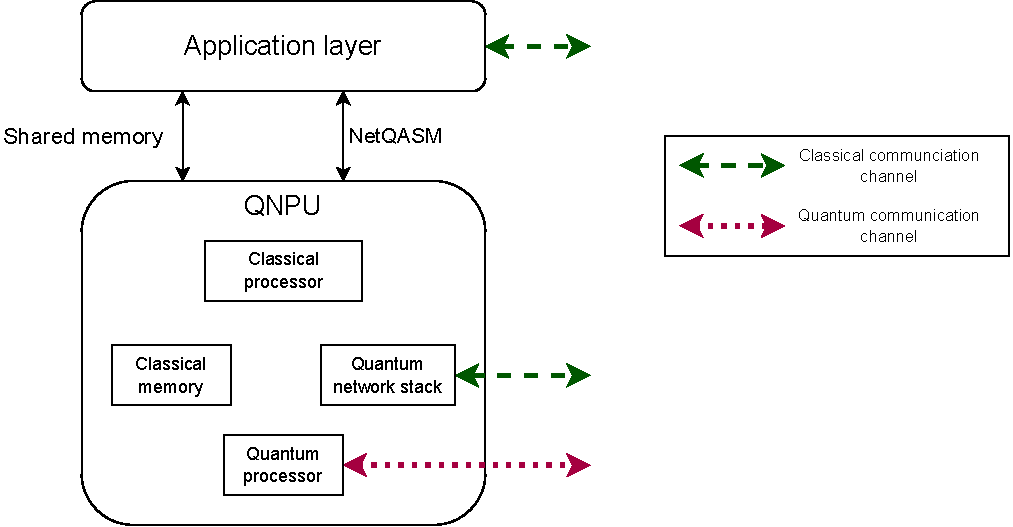
\includegraphics[width=0.7\textwidth]{figures/netqasm/qnpu.pdf}
    \caption{Overview of \ac{QNPU} components and interfaces. The \ac{CNPU} talks to
        the \ac{QNPU} using \ac{NetQASM}. The processor inside the \ac{QNPU} can interact with
        all other components. Channels are connecting components with corresponding
        components in adjacent nodes in the network.}
    \label{netqasm:fig:qnpu}
\end{figure}



\subsection{Applications and programs}
As also mentioned in~\cref{background:sec:applications}, quantum network \textit{applications} (or protocols) are multi-partite and distributed over multiple end-nodes.
The unit of code that is executed on each of the end-nodes that are part of the application, is called a \textit{program}.
We will use this terminology throughout the rest of this thesis.

As mentioned in the previous section, the end-nodes are modeled such that there is a \ac{CNPU} and a \ac{QNPU}. We assume that execution of quantum network programs is handled by the \ac{CNPU}.
How exactly the program is executed, and how the \ac{QNPU} is involved herein, is part of the \ac{NetQASM} proposal.
\section{Use-cases}
\label{netqasm:sec:use_cases}
In the next section we will discuss the design considerations taken when developing \ac{NetQASM}.
These design considerations are based on a set of use-cases listed in this section which we intend for \ac{NetQASM} to support.
Applications intended to run on a quantum network will often depend on a combination of these use-cases.

\begin{itemize}
      \item \textbf{Local quantum operations}.
            Applications running on a network node need to perform quantum operations on local qubits, including initialization, measurement, and single- or multi-qubit gates.
            Such local qubit manipulation is well known in the field of quantum computing. For example, OpenQASM~\cite{cross2017openqasm} describes quantum operations.
            Quantum \textit{network} applications should be able to do these local operations as well.

      \item \textbf{Local quantum operations depending on local events or data}.
            The next use-case stems from applications consisting of programs in which limited classical computation or decision making is needed in-between performing quantum operations.
            Here we consider only dependencies in a program between quantum operations and information that is produced locally, that is, on the node that this program is being executed.
            For instance, a program might only apply a quantum gate on a qubit depending on the measurement outcome of another qubit, or choose between execution branches based on evaluation of a classical function of earlier measurement outcomes.
            An example is for the server-side of \textit{blind quantum computation}, which performs a form of Measurement-Based Quantum Computation (MBQC).
            In each step of the MBQC, the server performs certain gates on a qubit, depending on results of measuring previous qubits~\cite{fitzsimons2017private}.
            These applications need classical operations to not take too much time, so that qubit states stay coherent during these operations.
            This implies that switching between classical and quantum operations should have little overhead.

      \item \textbf{Entanglement generation}.
            Crucial to quantum networks is the ability to generate remote \textit{entanglement}.
            Applications should be able to specify requests for entanglement generation between remote nodes.
            In some cases, a Measure-Directly (MD)~\cite{dahlberg2019linklayer} type generation is required, where entangled state is measured directly, without storing in memory, to obtain correlated classical bits, such as in Quantum Key Distribution (QKD).
            However, in many cases a Create-Keep (CK)~\cite{dahlberg2019linklayer} type is needed, where the entanglement needs to be stored in memory and further operations applied involving other qubits.
            We want applications to be able to \textit{initiate} or \textit{receive} (await) entanglement of both forms with nodes in the network.

      \item \textbf{Local quantum operations depending on remote events or data}.
            We already mentioned the use-case of having conditionals based on \emph{local} information.
            We also envision applications that need to store qubits and subsequently perform local quantum operations on them and other local qubits, based on classical information coming from \textit{another node}.
            An example is \textit{teleportation} in which the receiver---after successful entanglement generation---needs to apply local quantum corrections based on the measurement outcomes of the sender.
            Another application is blind quantum computation, where the server waits for classical instructions from the client about which quantum operations to perform.
            Hence, there need to be integration of classical communication (sending the measurement results or further instructions) and the local quantum operations.
            Furthermore, since classical communication has a non-zero latency (and is in general even non-deterministic), it should be possible to suspend doing quantum operations while waiting for communication or performing classical processing, while quantum states stay coherent.


      \item \textbf{Waiting time}.
            We consider the scenario where an application requires two nodes to communicate with each other, and where communication takes a long time, for example since they are physically far apart.
            It should be possible for a program to suspend doing quantum operations while waiting for communication or performing classical processing, while quantum states stay coherent.
            Furthermore, in order to maximize the usage of the \ac{QNPU} we want to have a way to fill this waiting time in a useful way.
\end{itemize}
\section{Design Considerations}
\label{netqasm:sec:design_considerations}
In this section we review the most important design considerations and requirements that were applied when
developing \ac{NetQASM}.
Our proposed solutions to these design considerations are presented in the next section, with more details about \ac{NetQASM} as a language
in the subsequent sections.

\begin{itemize}
      \item \label{item:design_ent_gen} \textbf{Remote entanglement generation:}
            One of the main differences compared to the design considerations of a quantum computing architecture is that of remote entanglement
            generation (see the use-case in~\cref{netqasm:sec:use_cases}).
            Nodes need to be able to generate entanglement with a remote node, which requires the collaboration and synchronization of both nodes, and possibly intermediate nodes, which is handled by the network stack (\cref{netqasm:sec:abstract_model}).

            Further requirements arise in platforms with a limited number of communication qubits.
            The extreme case is nitrogen-vacancy centers in diamond which have a single communication qubit that additionally is required for performing local operations.
            For this reason it is not possible to decouple local gates on qubits from entanglement
            generation.
            We note the contrast with classical processors, where networking operations are typically intrinsically separate kinds of operations.
            For example, operations such as sending a message may simply involve moving data to a certain memory (e.g. that of a physically separate network interface), which is often abstracted as a system call.

            A quantum network stack has already been proposed in~\cite{dahlberg2019linklayer,kozlowski2020networklayer}, and we expect the \ac{QNPU} of the end-node to implement such a stack, including a \textit{network layer} that exposes an interface for establishing entanglement with remote nodes.
            The way in which a program creates remote entanglement should therefore be compatible with this network layer.

      \item \label{item:design_cond} \textbf{Conditionals:}
            In~\cref{netqasm:sec:use_cases} we mentioned the need to do local quantum operations conditioned on classical data that may be generated locally or by remote nodes. Such classical data include for example measurement results or information communicated to or from other nodes in the network.
            We distinguish between real-time and near-time conditionals~\cite{cross2021openqasm}.
            Real-time conditionals are time-sensitive, such as applying a certain quantum operation on a qubit depending on a measurement outcome.
            For such conditionals, we would like to have fast feedback, in order for quantum memory not to wait too long (which would decrease their quality).
            Near-time conditionals are not as sensitive to timing.
            For example, a program may have to wait for a classical message of a remote node, while no quantum memory is currently being used.
            Although it is preferably minimized, the actual waiting time does not affect the overall execution quality.


      \item \label{item:design_return} \textbf{Shared memory:}
            As described in \cref{netqasm:sec:abstract_model}, we expect end-nodes to consist of an application layer and a \ac{QNPU}.
            These two components have different capabilities.
            For example, only the application layer has the ability to do arbitrary classical communication with other nodes.
            Only the \ac{QNPU} can do quantum operations.
            These restrictions lead the design in a certain way.
            The two components hence need to work together somehow.
            There needs to be model for interaction between the two, and also for shared memory.

            Executing programs on an end-node is shared by the application layer and the \ac{QNPU} (see~\cref{netqasm:sec:abstract_model}).
            Indeed, only the \ac{QNPU} can do quantum-related operations, whereas the application layer needs to do classical communication.
            In order to make these work together, the two components have to share data somehow.
            This includes the application layer requesting operations on the \ac{QNPU}, and sending the following from the \ac{QNPU} to the \ac{CNPU}:
                (1) measurement outcomes of qubits,
                (2) information about entanglement generation, in particular a way to identify entangled pairs.
            This communication between \ac{CNPU} and \ac{QNPU} needs to be done during runtime of the program.
            This is in contrast to local quantum computation, where one might wait until execution on the \ac{QNPU} is finished before returning all data.
            The challenge for quantum network programs is to have a way to return data while quantum memory stays in memory.

      \item \textbf{Processing delay:}
            Since we assume that the application layer and the \ac{QNPU} have to share execution of a single program, the interaction between the two layers should be efficient.
            Unnecessary delays lead to reduced quality (see~\cref{netqasm:sec:introduction}).
            The challenge is therefore to come up with an architecture for the interaction between the application layer and the \ac{QNPU}, as well as a way to let \ac{QNPU} execution not take too long.
      \item \textbf{Platform-independence:}
            As explained in~\cref{netqasm:sec:introduction}, hardware can have many different capabilities and gates that can be performed.
            However, application programmers should not need to know the details of the underlying hardware.
            For this reason, there needs to be a framework through which a programmer can develop an application in a platform-independent way which compiles to operations the \ac{QNPU} can execute.
      \item \textbf{Potential for optimization:}
            Since near-term quantum hardware has a limited number of qubits and qubits have a relatively short lifetime, the hardware should be utilized in an effective way.
            There is therefore a need to optimize the quantum gates to be applied to the qubits.
            This includes for example choosing how to decompose a generic gate into native gates, rearranging the order of gates and measurements and choosing what gates to run in parallel.
            Since different platforms have vastly different topologies and gates that they can perform, this optimization needs to take the underlying platform into account.
            The challenge is to have a uniform way to express both platform-independent and platform-specific instructions.
      \item \textbf{Multitasking:}
            The `Waiting time' use-case in~\cref{netqasm:sec:use_cases} describes that a node's \ac{QNPU} may have to wait a long time. We consider the solution that the \ac{QNPU} may do multitasking, that is, run multiple (unrelated) programs at the same time.
            Then, when one program is waiting, another program can execute (partly) and fill the gap.
            To make our design compatible with such multitasking, we need to provide a way such that programs can run at the same time as other programs, but without having to know about them.
      \item \textbf{Ease of programming:}
            Even though \ac{NetQASM} provides an abstraction over the interaction with the \ac{QNPU}, it is still low-level and hence not intended to be used directly by application developers.
            Furthermore, applications also contain classical code that is not intended to run on the \ac{QNPU}.
            Therefore it should be possible to write programs consisting of both classical and quantum (network) operations in a high-level language like Python, and compile them to a hybrid quantum-classical program that uses \ac{NetQASM}.

\end{itemize}
\section{Design Decisions}
\label{netqasm:sec:design_decisions}

Based on the use-cases, design considerations and requirements, we have designed the low-level language \ac{NetQASM} as an API to the \ac{QNPU}.
In this section we present concepts and design decisions we have taken.
Details on the mode of execution and the \ac{NetQASM}-language are presented in \cref{netqasm:sec:implementation}.

\subsection{Interface between \ac{CNPU} and QNPU}
\label{netqasm:sec:design_decisions_interface}

\subsubsection{Execution model}
As described in \cref{netqasm:sec:abstract_model}, and also in \cref{netqasm:sec:design_considerations} program execution is split across the \ac{CNPU} and the \ac{QNPU}.
Since the \ac{QNPU} is assumed to have limited processing power (\cref{netqasm:sec:abstract_model}), our design lets the \ac{CNPU} do most of the classical processing.
The program blocks (\cref{fig:program_decomp}) are hence spread over two separate systems: blocks of purely classical code are executed by the \ac{CNPU}, and blocks of quantum code (containing both quantum operations and limited classical control) are executed by the \ac{QNPU}.

The quantum code (including limited classical control) is expressed using the \ac{NetQASM} language.
The classical code is handled completely by the \ac{CNPU}, and we do not impose a restriction to its format.
In our implementation (\cref{netqasm:sec:python-sdk}), we use Python.
This classical code on the \ac{CNPU} also handles all application-level classical communication between nodes, since it cannot be done on the \ac{QNPU}.

We let the \ac{CNPU} initiate a program.
Whenever quantum code needs to be executed, the \ac{CNPU} delegates this to the \ac{QNPU}.
Since processing delay should be minimized (\cref{netqasm:sec:design_considerations}), the communication between \ac{CNPU} and \ac{QNPU} should be minimized.
Therefore, \ac{NetQASM} bundles the quantum operations together into blocks of instructions, called \textit{subroutines}, to be executed on the \ac{QNPU}.
A program, then, consists of both both classical code and quantum code, and the quantum code is represented as one or more subroutines.
These subroutines can be seen as the quantum code blocks of~\cref{fig:program_decomp}.

For most programs, we consider subroutines to be sent consecutively in time.
However, if the \ac{QNPU} supports it, \ac{NetQASM} also allows to send multiple subroutines to be executed on the \ac{QNPU} at the same time, although this requires some extra care when dealing with shared memory.
From the perspective of the \ac{QNPU}, a program consists of a series of subroutines sent from the \ac{CNPU}.
Before receiving subroutines, the \ac{CNPU} first \textit{registers} a program at the \ac{QNPU}.
The \ac{QNPU} then sets up the classical and quantum memories (see below) for this program.
Then, the \ac{CNPU} may send subroutines to the \ac{QNPU} for execution.


\subsubsection{Shared classical memory}
Since classical and quantum blocks in the code (as per \cref{fig:program_decomp}) can depend on each other, the \ac{CNPU} and the \ac{QNPU} need to have a way to communicate information to each other.
For example, a subroutine may include a measurement instruction; the outcome of this measurement may be used by the \ac{CNPU} upon completion of the subroutine.
Therefore, \ac{NetQASM} uses a shared memory model such that conceptually both layers can access and manipulate the same data. This solves the need to return data, and to do conditionals (\cref{netqasm:sec:design_considerations}).

Each program has a classical memory space consisting of \textit{registers} and \textit{arrays}.
Registers are the default way of storing classical values, like a measurement outcome.
In the example of the \ac{CNPU} needing a measurement outcome, there would be an instruction in the subroutine saying that a measurement outcome needs to be placed in a certain register.
The \ac{CNPU} can then access this same register (since they share the memory space) and use it in further processing.
The number of registers is small, and constant for each program.
Arrays are collections of memory slots (typically the slots are contiguous), which can be allocated by the program at runtime.
Arrays are used to store larger chunks of data, such as parameters for entanglement requests, entanglement generation results, or multiple measurement outcomes when doing multiple entangle-and-measure operations.
The \ac{CNPU} may only read from the shared memory; writing to it can only be done by issuing \ac{NetQASM} instructions such as \texttt{set} (for registers) and \texttt{store} (for arrays).
The \ac{QNPU} may directly write to the shared memory, for example when entanglement finished and it writes the results to the array specified by the program.


\begin{figure}[t]
      \centering
      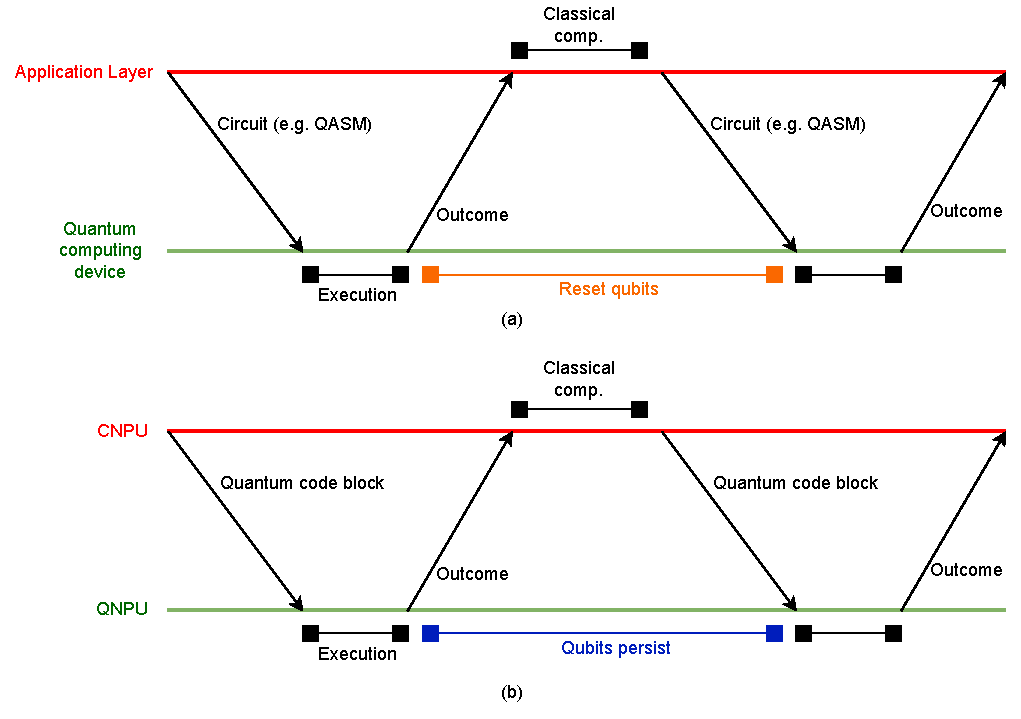
\includegraphics[width=0.8\linewidth]{figures/netqasm/classical-quantum-interaction.pdf}
      \caption{Program interaction between the \ac{CNPU} and a quantum device in
            both the case of \emph{hybrid-quantum computing} (a)
            and quantum networks (b). In the case of hybrid-quantum
            computing, qubits are reset in between circuits (in e.g. QASM). For
            quantum internet programs the qubits should on the other hand be
            kept in memory, since they might be entangled with another node and
            intended to be used further.}
      \label{fig:hybrid}
\end{figure}

\subsubsection{Unit modules}
In order to support systems with multitasking (\cref{netqasm:sec:design_considerations}), \ac{NetQASM} provides a virtualized model of the quantum memory to the program.
This allows the \ac{QNPU} to do mapping between the virtualized memory and the physical memory and perform scheduling between programs.

The quantum memory for a program is represented by a \textit{unit module} (\cref{fig:topology}).
A unit module defines the topology of the available qubits (which qubits are connected, i.e. on which qubit pairs a two-qubit gate can be executed), plus additional information on each qubit.
This additional information consists of which gates are possible on which qubit or qubit pair.
It also specifies if a qubit can be used for remote entanglement generation or not.
The extra information is needed since on some platforms, not all qubits can be used for entanglement generation and different qubits may support different local gates.
For example, in a single NV-centre, there is only one communication qubit and any additional qubits are storage qubits.
Also, the communication qubit can do different local gates than the storage qubits.

A single program has a single quantum memory space, which is \textit{not} reset at the end of a subroutine, which is in contrast with quantum computing.
This allows the \ac{CNPU} to do processing while qubits are in memory.
The following sequence of operations provides an example.
    (1) The \ac{CNPU} first sends a subroutine containing instructions for entanglement generation with a remote node R.
    (2) The \ac{QNPU} has finished executing the subroutine, and informs the \ac{CNPU} about it.
        There is now a qubit in the program's memory that is entangled with some qubit in R.
    (3) The \ac{CNPU} does some classical processing and waits for a classical message from (the \ac{CNPU} of) R.
    (4) Based on the contents of the message, the \ac{CNPU} sends a new subroutine to the \ac{QNPU} containing instructions to do certain operations on the entangled qubit.
        The subroutine can indeed access this qubit by using the same identifier as the first subroutine, since the quantum memory is still the same.
        We note the contrast with (non-network) quantum computing, where quantum memory is reset at the end of each block of instructions (\cref{fig:hybrid}).


Unit modules contain \textit{virtual qubit IDs}.
This is because of the requirement that it should be possible to run multiple programs at the same time on a single \ac{QNPU} (Multitasking consideration in \cref{netqasm:sec:design_considerations}).
We use an approach that is similar to virtual memory in classical systems~\cite{arpaci2018operating}.
Each application has control over a set of physical qubits, but the application does not (need to) know which physical qubits these are exactly.
The unit module provides a virtualized view of this available memory.
This view contains virtual IDs each representing a single qubit, called a virtual qubit.
The \ac{QNPU} maintains a mapping of virtual IDs (per application) to physical qubits.
The \ac{QNPU} may change this mapping over time, without the applications knowing.
We stress that our virtualization hence only involves a mapping from IDs to physical qubits.
There is no copying of quantum states involved.

We note that this design decision meets our Multitasking consideration(\cref{netqasm:sec:design_considerations}).
By using virtualized unit modules, the \ac{QNPU} is free to map qubit IDs of the application to physical qubits as it sees fit.
For example, consider a node with a physical memory consisting of one communication qubit, and multiple memory qubits.
Application A creates entanglement with a remote node such that its half of the pair is in the communication qubit.
Then, application A needs to wait for a long time before further processing the quantum state in this qubit, for example since it needs to wait for a classical message from a remote node.
Meanwhile, application B is waiting to be executed on the \ac{QNPU}, and it also requires the communication qubit for entanglement generation.
The \ac{QNPU} can now move the state from the communication qubit to one of the memory qubits, and update the mapping of application A's ID to this physical memory qubit.
Then, the \ac{QNPU} can run application B while A is waiting for the classical message.
When B has finished, the \ac{QNPU} can move A's state back to the communication qubit.
Since application A uses the unit module and does not know about the physical memory, it
    (1) does not care that its state was temporarily moved to a different physical qubit, and
    (2) can remain oblivious about any other application being run (like B) while it is waiting.


\begin{figure}[t]
      \centering
      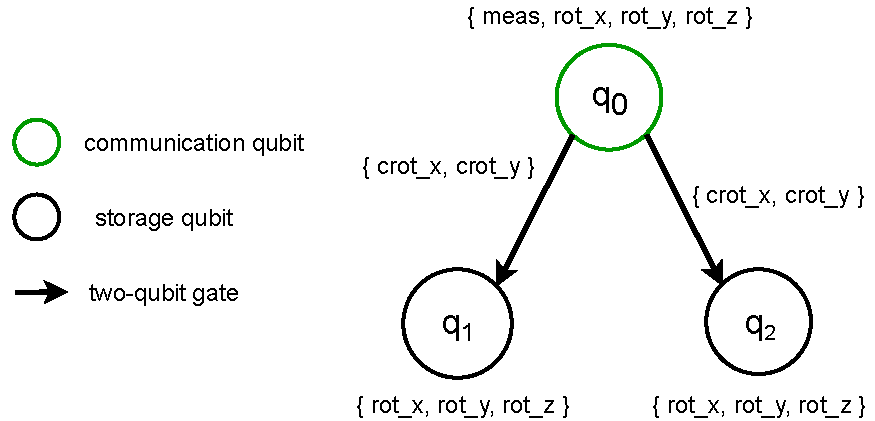
\includegraphics[width=0.6\linewidth]{figures/netqasm/unit-module.pdf}
      \caption{Example of a unit-module topology on a platform using
            nitrogen-vacancy centers in diamond. A unit-module is a
            hypergraph~\cite{berge1984hypergraphs}, with associated information
            on both nodes and edges. Each node represents a virtual qubit,
            containing information about (1) its qubit type (communication or
            storage), (2) physical properties of the qubit, such as decoherence
            times and (3) which single-qubit gates are supported on the qubit,
            together with their duration and noise. Each edge represents the
            possibility of performing joint operations on those qubits, such as
            two-qubit gates, and also containing information about gate
            durations and noise.}
      \label{fig:topology}
\end{figure}



\subsection{NetQASM language}

\subsubsection{Instructions}
\label{netqasm:sec:design_decisions_language}
As explained in~\cref{netqasm:sec:design_decisions_interface}, the \ac{CNPU} delegates quantum code (including limited classical control) of the program to the \ac{QNPU} by creating blocks of instructions and sending these to the \ac{QNPU} for execution.
These blocks are called subroutines and contain \ac{NetQASM} \textit{instructions}.
Since the \ac{QNPU} is meant to be limited in processing power, the instruction set that it interprets should also be simple and low-level.
The \ac{NetQASM} instruction set contains instructions for simple arithmetic, classical data manipulation, and simple control flow in the form of (un)conditional branch instructions.
Although conditional control-flow can be done at the \ac{CNPU} as well, \ac{NetQASM} branching instructions allow for much faster feedback since they are executed by the \ac{QNPU}, and hence cover the design consideration of real-time conditionals (\cref{netqasm:sec:design_considerations}).
We note the obvious performance gain by being able to do control logic without having to go back to the \ac{CNPU}.
There are no higher-level concepts such as functions or for-loops, which would require more complicated and resource-demanding parsing for the \ac{QNPU}, such as constructing an abstract syntax tree.

A single instruction specifies an operation, possibly acting on classical or quantum data.
For example, a single-qubit rotation gate is represented as an instruction containing the type of gate, the classical register containing the rotation angle, and the classical register containing the virtual ID of the qubit (as specified in the unit module) to act on.
\ac{NetQASM} specifies a set of \textit{core} instructions that are expected to be implemented by any \ac{QNPU}.
These include classical instructions like storing and loading classical data, branching, and simple arithmetic.
Different hardware platforms support different quantum operations.
\ac{NetQASM} should also support platform-specific optimization (\cref{netqasm:sec:design_considerations}).
Therefore, \ac{NetQASM} uses \textit{flavors} of quantum instructions (\cref{netqasm:sec:design_decisions_flavours}).
The \textit{vanilla} flavor consists universal of a set of platform-independent quantum gates.
Particular hardware platforms, such as the NV-centre, may use a special NV flavor, containing NV-specific instructions.
A \ac{QNPU} implementation may use a custom mapping from vanilla instructions to platform-specific ones.
The instructions in a flavor are also called a software-visible gate set~\cite{murali2019fullstack}.
See~\cref{netqasm:sec:instructions} for more details on \ac{NetQASM} instructions.

\subsubsection{Remote entanglement generation}
Generating entanglement with a remote node is also specified by instructions.
These are however somewhat special compared to other instructions.
First, entanglement generation has a non-deterministic duration.
Therefore, when an entanglement instruction is executed, the request is forwarded to the part of the system responsible for creating entanglement, but the instruction itself immediately returns.
A separate \textit{wait} instruction can be used to block on entanglement generation to actually be completed.
Second, entanglement generation requests should be compatible with the network stack proposed in~\cite{dahlberg2019linklayer}, including the network layer from~\cite{kozlowski2020networklayer}.
These requests need to be accompanied by information such as the number of EPR pairs to generate or the minimum required fidelity.
Third, this information should be able to depend on runtime information.
For example, the required fidelity may depend on an earlier measurement outcome.
Therefore, entanglement generation parameters cannot be static data, and must be stored in arrays.
Furthermore, the result of entanglement generation with the remote node consists of a lot of information, such as which Bell state was produced, the time it took, and the measurement results in case of measuring directly.
This information is written by the \ac{QNPU} to an array which is specified by the entanglement instruction.
Finally, since writing the information to the array indicates that entanglement generation succeeded, the wait instruction can be used to wait until a certain array is filled in, such as the one provided by the entanglement instruction.
Since the entanglement instruction is non-blocking, it is possible to continue doing local operations while waiting for entanglement generation to complete.

We assume that the \ac{QNPU} implements a network stack where connections need to be set-up between remote nodes before entanglement generation can happen~\cite{kozlowski2020networklayer, dahlberg2019linklayer}.
\ac{NetQASM} provides a way for programs to open such connections in the form of \textit{EPR sockets}.
The \ac{CNPU} can ask the \ac{QNPU} to open an EPR socket with a particular remote node.
The \ac{QNPU} is expected to set up the required connections in the network stack, and associates this program socket with the connection.
When the program issues an instruction for generating entanglement, it refers to the EPR socket it wants to use.
Based on this, the \ac{QNPU} can use the corresponding connection in the network.


\begin{figure}[t]
      \centering
      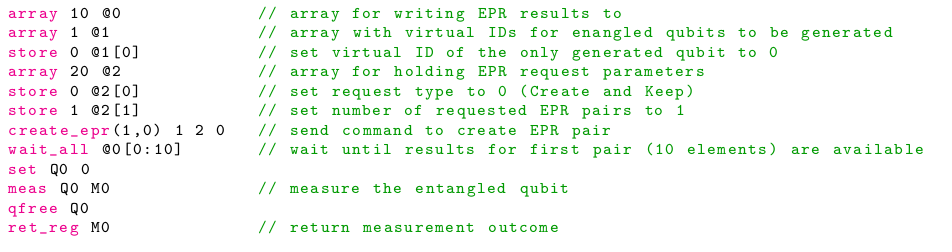
\includegraphics[width=0.6\linewidth]{figures/netqasm/nqasm_code_example}
      \caption{Example of NetQASM code for generating a single entangled pair with another node followed by a measurement.
            See the Appendix for more details of the instructions.}
      \label{fig:nqasm_code_example}
\end{figure}

\subsubsection{Flavors}
\label{netqasm:sec:design_decisions_flavours}
We want to keep \ac{NetQASM} platform-independent.
However, we also want the potential for platform-specific optimization (\cref{netqasm:sec:design_considerations}).
Therefore we introduce the concept of \textit{flavors}.
Flavors only affect the quantum instruction set of the language, and not the memory model or the interaction with the \ac{QNPU}.
We use the \textit{vanilla} or generic flavor for a general, universal gate set.
Subroutines may be written or generated in this vanilla flavor.
Platform-independent optimization may be done on this level.
A \ac{QNPU} may directly support executing vanilla-flavored \ac{NetQASM}.
Platform-specific translations may then be done by the \ac{QNPU} itself.
It can also be that a \ac{QNPU} only supports a specific flavor of \ac{NetQASM}.
A reason for this could be that the \ac{QNPU} does not want to spend time translating of the instructions at runtime.
In this case, the \ac{CNPU} should perform a translation step from the vanilla flavor to the platform-specific flavor.
In such a case, the vanilla flavor can be seen as an \textit{intermediate representation}, and the translation to a specific flavor as a back-end compilation step.

\subsubsection{Programmability}
Since the \ac{NetQASM} instructions are relatively low-level, we like to have a higher-level programming language for writing programs, that is automatically compiled to \ac{NetQASM}.
We introduce a higher-level SDK in \cref{netqasm:sec:python-sdk}.
However, we do not see this as part of the \ac{NetQASM} specification itself.
This decoupling allows the development of SDKs to be independent such that these can be provided in various languages and frameworks.

We still want \ac{NetQASM} instructions to be suitable for manual writing and inspection.
Therefore, instructions (and subroutines) have two formats: a binary one that is used when sending to the \ac{QNPU}, and a text format that is human-readable.
The text format resembles assembly languages including OpenQASM.
Examples are given in \cref{netqasm:sec:python-sdk} and the Appendix.
\section{Implementation}
\label{netqasm:sec:implementation}

\subsection{Interface between \ac{CNPU} and \ac{QNPU}}
Here we explain the flow of messages between the \ac{CNPU} and the \ac{QNPU}.
The \ac{CNPU} starts by declaring the registration of an application, including resource-requirements for the application.
After this, the \ac{CNPU} sends some number of subroutines for the \ac{QNPU} to execute before declaring the application is finished.
See \cref{fig:message_sequence} for a sequence diagram and below for a definition of the messages.
In \cref{netqasm:sec:language} we will describe in more details the content of the subroutines and the format of instructions.
The \ac{QNPU} returns to the \ac{CNPU} an assigned application ID for the registered application and returns data based on the subroutines executed.

The \ac{CNPU} and the \ac{QNPU} are assumed to run independently and in parallel.
For example, while a subroutine is being executed by the \ac{QNPU}, the \ac{CNPU} could in principle do other operations, such as heavy processing or communication with another node.

\begin{figure}
      \centering
      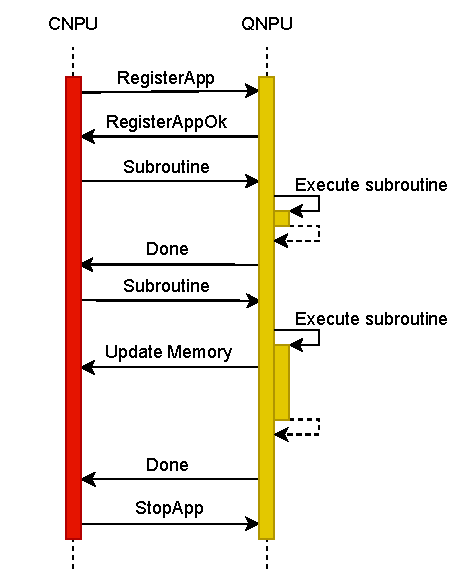
\includegraphics[width=0.5\linewidth]{figures/netqasm/message-flow.pdf}
      \caption{Flow of messages between the \ac{CNPU} and the \ac{QNPU}.}
      \label{fig:message_sequence}
\end{figure}

\Cref{fig:message_sequence} shows an example of a message exchange between the \ac{CNPU} and the \ac{QNPU}.
The content of these messages is further detailed in~\cref{netqasm:sec:app-messages}.



\subsection{The language}
\label{netqasm:sec:language}
The syntax and structure of \ac{NetQASM} resemble that of classical assembly languages, which in turn inspired the various QASM-variants for quantum computing~\cite{cross2017openqasm, khammassi2018cqasm, fu2019eqasm, liu2017fqasm}.

A \ac{NetQASM}-instruction is formed by an instruction name followed by some number of operands:
\begin{nqcode}
      instr operands
\end{nqcode}
where \nq{instr} specifies the instruction, for example \nq{add} to add numbers or \nq{h} to perform a Hadamard.
The \nq{operands} part consists of zero or more values that specify additional information about the instruction, such as which qubit to act on in the case of a gate instruction.
Instructions and operands are further specified in~\cref{netqasm:sec:operands}.

\subsection{Instructions}
\label{netqasm:sec:instructions}
There are eight groups of instructions in the \textbf{core} of \ac{NetQASM}.
Also summarized in \cref{fig:instructions}, these are:
\begin{itemize}
      \item \textbf{Classical:} Classical arithmetic on integers.
      \item \textbf{Branch:} Branching operations for performing conditional logic.
      \item \textbf{Memory:} Read and write operations to classical memory (register and arrays).
      \item \textbf{Allocate:} Allocation of qubits and arrays.
      \item \textbf{Wait:} Waiting for certain events. This can for example be the event that entanglement has been generated by the network stack.
      \item \textbf{Return:} Returning classical values from the \ac{QNPU} to the \ac{CNPU}.
            In our implementation we implement this by having the \ac{QNPU} write to the shared memory so that the \ac{CNPU} can access it.
      \item \textbf{Measurement:} Measuring a qubit.
      \item \textbf{Entanglement:} Creating entanglement with a remote node using the quantum network stack.
\end{itemize}

\begin{figure}
      \centering
      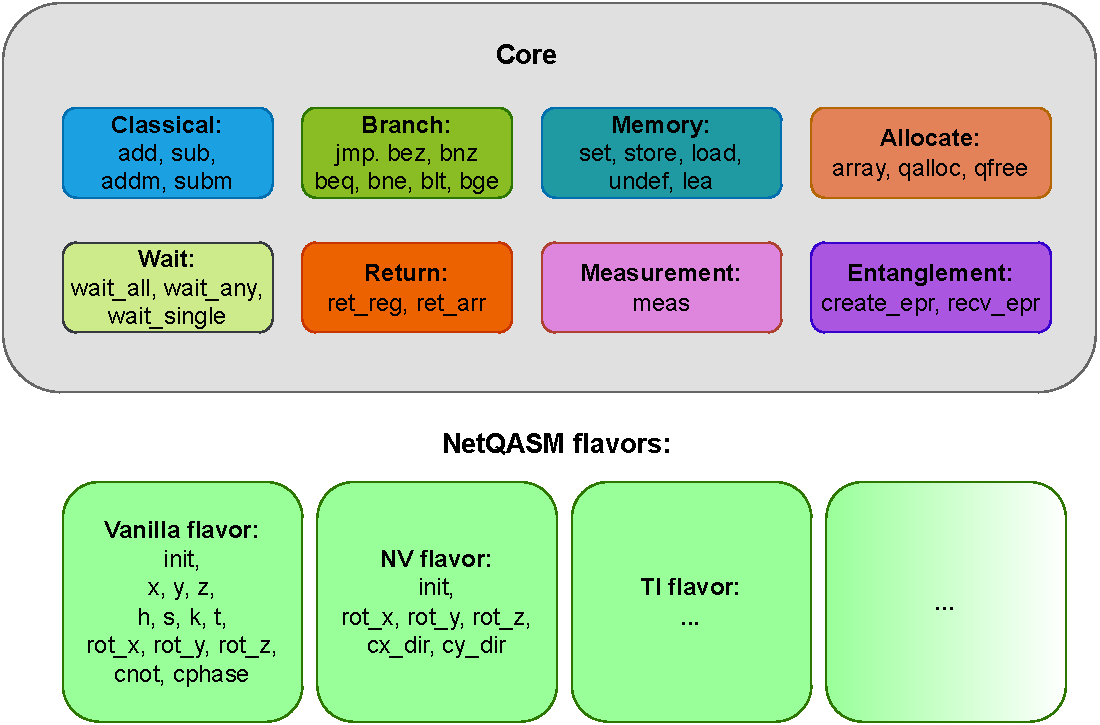
\includegraphics[width=0.8\linewidth]{figures/netqasm/instructions.pdf}
      \caption{The \textbf{core} of \ac{NetQASM} consists of eight groups of
            instructions. The quantum gates are defined as a set of software-visible
            gates part of a \ac{NetQASM} \textbf{flavor}. The \textbf{vanilla flavor}
            is the unique platform-independent \ac{NetQASM} \textbf{flavor} of
            \ac{NetQASM}, which can be used by a compiler.}\label{fig:instructions}
\end{figure}

Quantum gates are specific to a \ac{NetQASM} \textbf{flavor} and given as a set of software-visible gates of a given platform, see \cref{netqasm:sec:design_considerations}.
There is a single platform-independent \ac{NetQASM} \textbf{flavor} which we call the \textbf{vanilla flavor}, see \cref{fig:instructions}.
The \textbf{vanilla flavor} can be used as an intermediate representation for a compiler.


\subsection{Compilation}
Although application programmers could write \ac{NetQASM} subroutines manually, and let their (classical) application code send these subroutines to the \ac{QNPU}, it is useful and more user-friendly to be able to write quantum internet applications in a higher level language, and have the quantum parts compiled to \ac{NetQASM} subroutines automatically.
For this, we use the compilation steps depicted in \cref{fig:comp_chain}.
The format and compilation of the higher-level programming language is not part of the \ac{NetQASM} specification.
However, we do provide an implementation in the form of an SDK, see \cref{netqasm:sec:python-sdk}.

\begin{figure*}
      \centering
      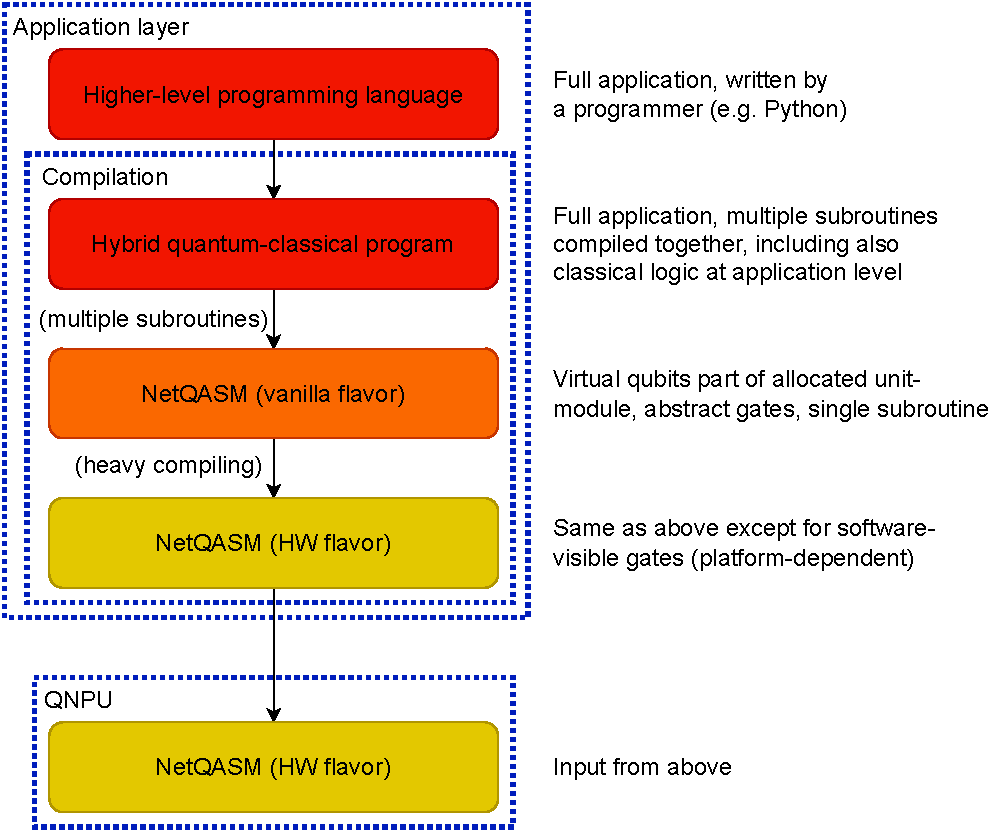
\includegraphics[width=0.7\linewidth]{figures/netqasm/comp-chain.pdf}
      \caption{Compilation steps from higher-level programming language, to the
            \ac{NetQASM} \textbf{flavor} exposed by the specific platform. What is
            contained at each level is further specified to the right of the
            diagram.}
      \label{fig:comp_chain}
\end{figure*}

\section{Python SDK}
\label{netqasm:sec:python-sdk}
We implemented \ac{NetQASM} by developing a Software Development Kit (SDK) in Python.
This SDK allows a programmer to write quantum network programs as Python code, including the quantum parts.
These parts are automatically translated to NetQASM subroutines.
The SDK contains a simulator that simulates a quantum network containing end-nodes, each with a \ac{QNPU}.
The SDK can execute programs by executing their classical parts directly and executing the quantum parts as \ac{NetQASM} subroutines on the simulated \ac{QNPU}.
By executing multiple programs at the same time, on the same simulated network, a whole multi-partite application can be simulated.
In~\cref{netqasm:sec:evaluation} we use this SDK to evaluate some of the design decisions of \ac{NetQASM}.

We refer to the docs at~\cite{git_netqasm} for the latest version of the SDK.
Below, we give an example of an application written in the SDK to give an idea of how development in the SDK looks like.
In \cref{app:examples_sdk} we provide a few more examples of applications in the SDK and their corresponding \ac{NetQASM} subroutines.

All code can be found at~\cite{git_netqasm} and~\cite{git_squidasm}, including:
    (1) Tools for serializing (de-serializing) to (from) both human-readable text form and binary encoding,
        % \item A parser for the human-readable form of \ac{NetQASM}.
        % \item A parser for binary encoding of \ac{NetQASM}.
        % \item An assembler of human-readable form to binary.
    (2) the \ac{NetQASM} SDK, together with compilers (no optimization yet),
    (3) support for running applications written in the SDK on the simulators NetSquid~\cite{netsquid,coopmans2021netsquid} and SimulaQron~\cite{dahlberg2018simulaqron}, and
    (4) implemented applications in \ac{NetQASM}, including: anonymous transmission~\cite{Christandl2005anonymous}, BB84~\cite{bb84}, blind quantum computing~\cite{broadbent2009universal,fitzsimons2017unconditionally}, CHSH game~\cite{Kaniewski2016}, performing a distributed CNOT~\cite{denchev2008distributed}, magic square game~\cite{brassard1999magicsquare}, teleportation~\cite{bennett1993teleporting}.

\subsection{SDK}
\label{netqasm:sec:sdk}
The SDK of \ac{NetQASM} uses a similar framework to the SDK used by the predecessor \ac{CQC}~\cite{git_cqc}.
Any program on a node starts by setting up a \texttt{NetQASMConnection} to the \ac{QNPU}-implementation in the \emph{backend}.
The \texttt{NetQASMConnection} encapsulates all communication that the \ac{CNPU} does with the \ac{QNPU}.
More information about supported backends can be found below in \cref{netqasm:sec:backends}.
Using the \texttt{NetQASMConnection} one can for example construct a \texttt{Qubit} object.
The \texttt{Qubit} object has methods for performing quantum gates and measurements.
When these methods are called, corresponding \ac{NetQASM} instructions are included in the current subroutine being constructed.
One marks the end of a subroutine, and the start of another, either by explicitly calling \texttt{flush} on the \texttt{NetQASMConnection} or by ending the scope of the \nq{with NetQASMConnection ...} context.

The following Python code shows a basic application written in the \ac{NetQASM} SDK.
The application will be compiled into a single subroutine executed on the \ac{QNPU}, which creates a qubit, performs a Hadamard operation, measures the qubit and returns the result to the application layer.
\subsubsection{Hello world/Hello Hadamard}
Functionally the same as the \ac{NetQASM}-subroutine~\ref{netqasm:sec:example_nq_hello_world}.
\begin{pycode}
  # Setup connection to backend
  # as the node Alice
  with NetQASMConnection("Alice") as alice:
    # Create a qubit
    q = Qubit(alice)
    # Perform a Hadamard on the qubit
    q.H()
    # Measure the qubit
    m = q.measure()
    # The end of the context also marks
    # the end of the subroutine
    # automatically but can also be done
    # explicitly using `alice.flush()`
\end{pycode}

The following \ac{NetQASM} subroutine is the result of translating the above Python code to \ac{NetQASM} of the vanilla (platform-independent) flavor.

\subsubsection{Hello world/Hello Hadamard}\label{netqasm:sec:example_nq_hello_world}
A simple subroutine which creates a qubit, performs a Hadamard, measures the qubit and returns the measurement outcome to the host.
\begin{nqcode}
  # NETQASM 1.0
  # APPID 0
  // Set the virtual qubit ID to use
  set Q0 0

  // Allocate and initialize a qubit
  qalloc Q0
  init Q0

  // Perform a Hadamard gate
  h Q0

  // Measure the qubit
  meas Q0 M0

  // Return the outcome
  ret_reg M0
\end{nqcode}

\subsubsection{Backends}
\label{netqasm:sec:backends}
As mentioned above, the \texttt{NetQASMConnection} in the SDK is responsible for communicating with the implemented \ac{QNPU} in the \emph{backend}.
The \emph{backend} can either be a simulator or an actual \ac{QNPU} using real quantum hardware.
Currently supported backends are the simulators SquidASM~\cite{git_squidasm} (using NetSquid~\cite{netsquid, coopmans2021netsquid}) and SimulaQron~\cite{dahlberg2018simulaqron}.
A physical implementation of \ac{QNPU} running on quantum hardware is being worked on at the time of writing.
Using the SDK provided at~\cite{git_netqasm}, one can for example simulate a set of program files for the nodes of a quantum network on NetSquid using a density matrix formalism with the command:
\begin{nqcode}
  netqasm simulate --simulator=netsquid --formalism=dm
\end{nqcode}
For more details see the docs at~\cite{git_netqasm}.
\section{Evaluation}
\label{netqasm:sec:evaluation}
We evaluate two of the design choices that we made for \ac{NetQASM}:
    (1) exposing unit-modules to the \ac{CNPU} and
    (2) adding the possibility to use platform-specific flavors of instructions.
For both elements we study the difference in including them in \ac{NetQASM} versus not including them.
We do this by simulating a teleportation application and a blind quantum computation application.
These examples also showcase the ability of \ac{NetQASM} to express general quantum internet applications.

We have implemented a simulator, called SquidASM~\cite{git_squidasm}, that simulates a network in which end-nodes have the internal architecture as described in~\cref{netqasm:sec:abstract_model}, that is, with an \ac{CNPU} and a \ac{QNPU}.
The simulator internally uses NetSquid~\cite{netsquid}, which was made specifically for the simulation of quantum networks.
SquidASM executes programs written using the SDK (\cref{netqasm:sec:python-sdk}), including sending \ac{NetQASM} subroutines to the (simulated) \ac{QNPU}.
The code and data that were used to produce the results in this section can be found at~\cite{git_netqasm_paper_data}.

We evaluate the performance of \ac{NetQASM} by looking at the runtime quality of two applications, both consisting of two programs (one per node).
The first is a teleportation of a single qubit from a sender node to a receiver node.
We define the quality as the fidelity between the original qubit state at the sender and the final qubit state at the receiver.
The second application is a blind computation protocol which involves a client and a server.
The server effectively performs, blindly, a single-qubit computation on behalf of the client.
The protocol is a so-called \textit{verifiable blind quantum computation}~\cite{fitzsimons2017unconditionally}.
This means that some of the rounds of the protocols are \textit{trap rounds}.
We define the quality that we evaluate as the error rate of these trap rounds, since this indicates the blindness of the server.

We run these applications on SquidASM, where we simulate realistic quantum hardware.
Specifically, we simulate nodes based on nitrogen-vacancies (NV) in diamond, that can do heralded entanglement generation between each other.
The simulated hardware uses noise models that are also used in~\cite{coopmans2021netsquid}.
For more details, see~\cref{netqasm:sec:simulation}.

A note on how we chose what to evaluate and what not.
We listed several design considerations in ~\cref{netqasm:sec:design_considerations}.
We addressed these in our design decisions (\cref{netqasm:sec:design_decisions}).
For some of these, it is straightforward to see how they address a certain consideration, such as conditionals allowing for fast runtime feedback, and unit modules for allowing multitasking, as explained in~\cref{netqasm:sec:design_decisions}.
Also, fundamental requirements like remote-entanglement generation and shared memory have been addressed.
The remaining considerations, and our solutions, namely platform independence and memory virtualization using unit modules, are less trivial to evaluate just by looking at the design.
Therefore, we focus on the evaluation of these two design decisions.

In our evaluation, we focus specifically on the Nitrogen-Vacancy hardware for our nodes.
This has two reasons.
First, it is a promising hardware platform for quantum network nodes~\cite{Taminiau2014} which we know quite well since it is available in the lab, and we have even used \ac{NetQASM} in a simple test case running on nodes based on NV~\cite{pompili2021experimental}.
Second, the NV hardware is interesting since it has a restricted gate set and qubit topology, which is explained in more detail below.
Therefore, we expect that the use of unit modules and an NV-specific flavor makes a difference in terms of runtime quality.

\subsection{Unit modules}
\label{netqasm:sec:evaluation-unit-modules}
We ask ourselves the question whether it pays off to expose unit modules, that is, a qubit topology with gate- and entanglement information.
Specifically, we want to know if there are situations where knowing the unit module gives the \ac{CNPU} an opportunity to optimize the application in a way that is not possible when not knowing the unit module.
If so, we are interested in how much advantage this gives (in terms of the runtime quality defined above).

In the next section we show that there are indeed situations where knowledge of the unit module is advantageous.
It can be that the order in which \ac{NetQASM} instructions are issued in a subroutine is sub-optimal, since virtual qubit IDs may be mapped in such a way that the \ac{QNPU} has to move virtual qubits to different physical qubits in order to execute the instructions.
If the \ac{CNPU} layer does not know this mapping, it cannot know that the instructions are ordered sub-optimally.
With knowledge of the unit module, on the other hand, the \ac{CNPU} can optimize the order and the overall application performance is improved.

We consider a teleportation application where a \textit{sender} program teleports a single qubit to another \textit{receiver} program.
It is assumed that the underlying platform is based on nitrogen-vacancy centers in diamond (NV) and use well-established models for both the noise and operations supported on such platforms, see \cref{netqasm:sec:simulation}.
The sender program uses two qubits: one to create entanglement with the receiver (qubit E), and one to send (teleport) to the receiver (qubit T).
At some point, the sender measures both qubits, after which it sends the outcomes to the receiver so that it can do the relevant corrections on its received qubit.
We assume that the sender program is written in a higher-level language like, like in our SDK (\cref{netqasm:sec:python-sdk}), and in such a way that it first issues a measurement operation on qubit T, and then on E. However, due to the differences in characteristics of the physical qubits, as will be explained below, it is more efficient to first do the measurement on E, and then on T. Now we consider two scenarios, namely
\begin{itemize}
  \item \textbf{Unit-modules (UM)}.
        We assume that the sender program is written and executed on a software stack implementing \ac{NetQASM}, which means that the application's view of its quantum working memory is in the form of a unit module.
        This unit module contains information about the above-mentioned hardware restrictions, and therefore a compiler can take advantage of it by re-ordering the measurement operations while generating the \ac{NetQASM} subroutines to be sent to the \ac{QNPU}.
  \item \textbf{No unit-modules (NUM)}.
        In this case the software stack also implements \ac{NetQASM}, but without unit modules.
        Specifically, the application sees its quantum memory as just a number of uniform qubits.
        Therefore, a compiler for this application does not know about the hardware restrictions, and will construct \ac{NetQASM}-subroutines sent to the \ac{QNPU} without doing any optimization and leaves the order of the operations to be performed as they are specified in the high-level SDK.
\end{itemize}

Let's first go through the steps of the teleportation application:\newline
\begin{description}
  \item[\textit{sender}]:
        \begin{enumerate}
          \item Initialize qubit $q_t$ to be teleported in a Pauli state.
          \item Create entanglement with \textit{receiver} using qubit $q_s$.
          \item Perform CNOT gate with $q_t$ as control and $q_s$ as target.
          \item Perform Hadamard gate on $q_t$.
          \item Measure qubit $q_t$ and store outcome as $m_1$.
          \item Measure qubit $q_s$ and store outcome as $m_2$.
          \item Send $m_1$ and $m_2$ to \textit{receiver}.
        \end{enumerate}
  \item[\textit{receiver}]:
        \begin{enumerate}
          \item Receive entanglement with \textit{sender} using qubit $q_r$.
          \item Receive measurement outcomes from \textit{sender}.
          \item Apply correction operations on $q_r$ based on measurement outcomes.
        \end{enumerate}
\end{description}

We will now consider the order of the steps of the \textit{sender}.
Firstly, we assume that the qubit to be teleported, $q_t$, is always created before the entanglement.
We motivate this assumption below. For this reason, steps 1--3 and 7 are fixed and cannot change.
However, we are free to do step 6 before step 4 and 5, since these single-qubit operations and measurements commute, as long as we are consistent with the outcomes $m_1$ and $m_2$.
Let's now consider what impact this decision of measuring $q_s$ before $q_t$ or not has on the quality of execution for a NV-platform.

One of the biggest restrictions on a NV-platform is the topology of the qubits.
In particular, the NV-platform has a single communication-qubit (electron) surrounded by some number of storage qubits (carbon spins), see for example \cref{netqasm:fig:topology}.
The single communication qubit is not only responsible for any remote entanglement generation but also for any two-qubit gate and is the only qubit that can be directly measured.
These restrictions require qubit states to be moved back and forth between the communication qubit and the storage qubits in order to free up the communication qubit, to create new entanglement or to measure another qubit.
Since the operation of moving a qubit state is relatively slow on this platform (up to a millisecond~\cite{Humphreys2018}) and adds noise to the qubits, it is important to try to minimize the number of moves needed.
For more details on the NV-platform, see for example~\cite{Bernien2014} or~\cite{dahlberg2019linklayer}.

In the steps of the \textit{sender} above, the communication qubit is first initialized to a Pauli state.
This state is then moved to a storage qubit to free up the communication qubit in order to create entanglement with the \textit{receiver}.
Then in step 5, $q_t$ should be measured, which is currently in the storage qubit.
This requires the qubit state to first be moved to the communication qubit.
However, at this point the communication qubit is occupied by the entangled pair and therefore first needs to be moved to a second storage qubit.
Qubit $q_t$ can then be moved to the communication qubit to be measured and then the same is done for $q_s$, requiring in total four move operations and three physical qubits.

We can now see that performing step 6 before 4 and 5 has the advantage that this qubit is already in the communication qubit and can be measured directly without moving it first.
Afterwards, $q_t$ can be moved to the communication qubit, which is cleared after the measurement, requiring in total only 2 move operations and only two physical qubits.
The decision of performing step 6 before 4 and 5 is highly dependent on the NV-platform and can only be made by a compiler that is aware about these restrictions.
The inclusion of unit-modules and qubit types in the \ac{NetQASM}-framework, which are exposed to the compiler at the \ac{CNPU}, allows for these optimization decision and can therefore improve the quality of execution.

For the two scenarios we consider, i.e. performing step 6 before 4 and 5 (\textbf{Unit modules (UM)}) or not (\textbf{No unit-modules (NUM)}), we check the average fidelity of the teleported state as a function of the gate noise (\cref{netqasm:fig:sweep_gate_noise}), as well as the average fidelity and execution time as a function of gate duration (\cref{netqasm:fig:sweep_gate_noise}), of the native two-qubit gate of the NV-platform. We see that performing step 6 before 4 and 5 improves both total execution time and average fidelity.
This can be explained by the fact that using unit modules allowed a compiler to produce \ac{NetQASM} code containing fewer two-qubit gates.
Therefore, an increase in two-qubit gate noise leads to a lower fidelity.
Also, an increase in two-qubit gate duration leads to higher execution time difference between the two scenarios.
Finally, \cref{netqasm:fig:sweep_gate_noise} shows that the two-qubit gate duration does not affect the final fidelity in this situation, but the difference between using unit modules versus not using them remains.


\begin{figure}[t]
    \centering
    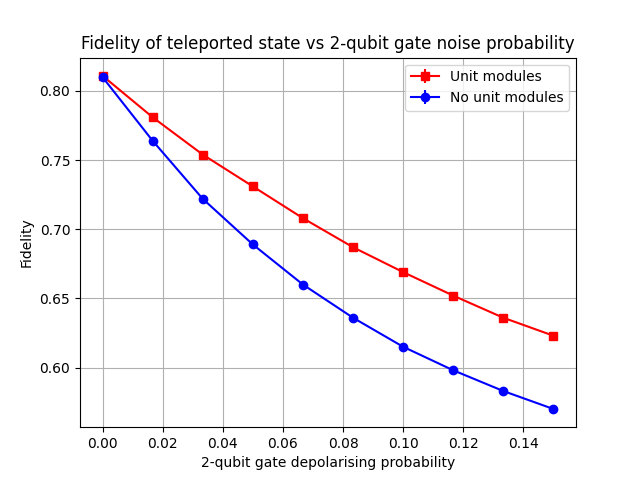
\includegraphics[scale=0.8]{figures/netqasm/plots/paper_teleport_sweep_gate_noise.png}
    \caption{
        Average fidelity between the original state at the sender and
        the final state at the server, as a function of the depolarizing noise
        of the native two-qubit gate of the NV-platform, both for the case of
        performing step 6 after (\textbf{No unit modules}) and before
        (\textbf{Unit modules}) step 4 and 5. Execution time of the native
        two-qubit gate is set to 0.5 ms. The rest of the parameters used are
        listed in \cref{netqasm:sec:simulation}. Each point is the average over each of
        the six Pauli states as initial state, repeated 100 times.}
    \label{netqasm:fig:sweep_gate_noise}
\end{figure}

\begin{figure}[t]
    \centering
    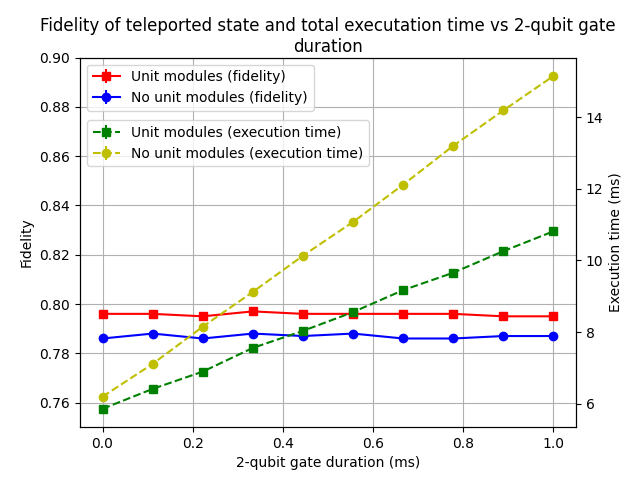
\includegraphics[scale=0.8]{figures/netqasm/plots/paper_teleport_sweep_gate_time.png}
    \caption{
        Average fidelity of the teleported state (left y-axis, solid lines) and total
        execution time of the teleportation application (right y-axis, dashed
        lines) as a function of the execution time of the native two-qubit gate
        of the NV-platform, both for the case of performing step 6 after
        (\textbf{No unit modules}) and before (\textbf{Unit modules}) step 4 and
        5. Dephasing parameter of the native two-qubit gate is set to 0.02. The
        rest of the parameters used are listed in \cref{netqasm:sec:simulation}. Each
        point is the average over each of the six Pauli state as initial state,
        repeated 100 times. In both figures, error bars are smaller than the drawn
        dots.}
  \label{netqasm:fig:sweep_gate_time}
\end{figure}



\subsection{Flavors}
\label{design_decisions_flavors}
While aiming to let \ac{NetQASM} be mostly platform-independent, we did also choose to allow platform-specific instructions, bundled in flavors.
The idea is that this allows for platform-specific optimization leading to better application performance.
Here we evaluate if flavors really impact potential performance, and if so how much.

We show that platform-specific optimization can indeed improve application performance, and that there are such optimizations that are not possible without flavors.
We see that it has impact mostly on the execution time, but not necessarily on outcome quality.

We consider the blind computation application depicted in \cref{netqasm:fig:bqc_app}, where both the client and server node implement the NV hardware.
Again we compare two scenarios, in this case:
\begin{itemize}
  \item \textbf{Vanilla}.
        We compile both the client's and server's application code to \ac{NetQASM} subroutines with the vanilla flavor.
        The \ac{QNPU}, controlling NV hardware which does not implement all vanilla gates natively, needs to translate the vanilla instructions on the go.
        We assume this translation is ad-hoc and does not do any optimizations like removing redundant gates.
  \item \textbf{NV}.
        The code is compiled to \ac{NetQASM} subroutines containing instructions in the NV flavor, and redundant gates are optimized away.
        The \ac{QNPU} can directly execute the instructions on the hardware.
\end{itemize}

We implemented this by writing two separate programs in the SDK, one for the client and one for the server.
The SDK automatically compiles the relevant parts of these programs into \ac{NetQASM} subroutines.
Classical communication (values $\delta_1$, $m_1$ and $\delta_2)$ is done purely between the two simulated \ac{CNPU}s, so these operations are not compiled to \ac{NetQASM} subroutines.
More details about the simulation can be found in \cref{netqasm:sec:simulation}.

The protocol is a verifiable blind quantum protocol~\cite{fitzsimons2017unconditionally}, which means that the circuit in~\cref{netqasm:fig:bqc_app} is run multiple times, namely once per round.
Some of these rounds are \textit{trap rounds} in which the client chooses a special set of input values.
Such a trap round can either succeed or fail, depending on the values returned by the server.
The fraction of trap rounds that fail is called the error rate.
The error rate should stay low in order for the computation to be blind.

We simulate the BQC application by running the client's and server's programs in SquidASM.
We look at the error rate of the trap round as a function of the two-qubit gate noise.
The result can be seen in~\cref{netqasm:fig:plot_bqc}.
It can be seen that using the NV flavor provides a better (lower) error rate than using the vanilla flavor.
This can be explained by noting that \ac{NetQASM} instructions in the vanilla flavor are mapped ad-hoc to native NV gates by the \ac{QNPU} at runtime, which leads to more two-qubit gates in total.


\begin{figure}[t]
  \centering
  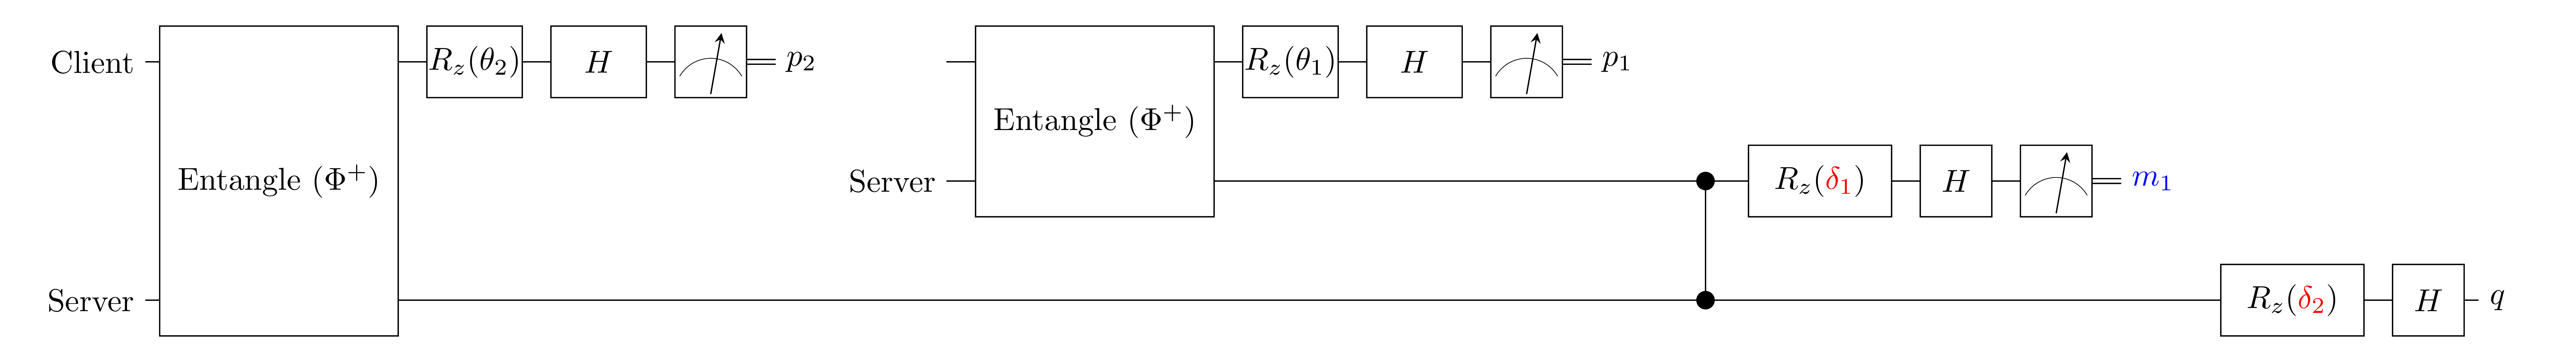
\includegraphics[width=0.6\linewidth]{figures/netqasm/bqc_app.png}
  \caption{Circuit representation of the simulated BQC application. The client
    remotely prepares two qubits on the server, by twice creating an
    entangled pair with the server followed by a local measurement. The
    server locally entangles its two qubits (cphase gate). Then, the client
    and server use classical communication to further guide the server's
    quantum operations. The client computes $\delta_1 = \alpha - \theta_1 +
      p_1 \cdot \pi$ and sends this to the server. The server uses the
    received value to do a local rotation and later sends measurement
    outcome $m_1$ back to the client. The client then sends $\delta_2 =
      (-1)^{m_1} \cdot (\beta - \theta_2 + p_2 \cdot \pi)$ to the server.
    The qubit state $q$ is the result of this application.
  }
  \label{netqasm:fig:bqc_app}
\end{figure}


\begin{figure}[t]
  \centering
  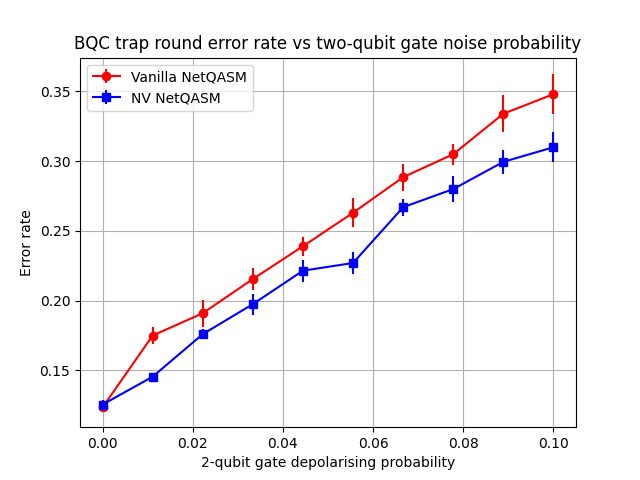
\includegraphics[scale=0.8]{figures/netqasm/plots/bqc_sweep_gate_noise_trap.png}
  \caption{
    Average error rate of trap rounds for the circuit of~\cref{netqasm:fig:bqc_app}.
    Each point is the average over four combinations of $\theta_1$ and $\theta_2$,
    each used in 500 trap rounds. It can be seen that using the vanilla (platform-independent)
    \ac{NetQASM} flavor results in a worse (higher) error rate on average.}
  \label{netqasm:fig:plot_bqc}
\end{figure}

To gain some more insight into why using the NV flavor provides a lower error rate we also look at the fidelity of the two quantum states on the server before any local gates are applied.
As can be seen in~\cref{netqasm:fig:bqc_app}, the client remotely prepares two states on the server by twice creating entanglement and measuring its own half of the EPR pair.
In~\cref{netqasm:fig:plot_bqc_fidelity} we see that already during this remote state preparation phase the NV flavor outperforms the vanilla flavor in terms of the fidelity of the prepared states.

\begin{figure}[t]
  \centering
  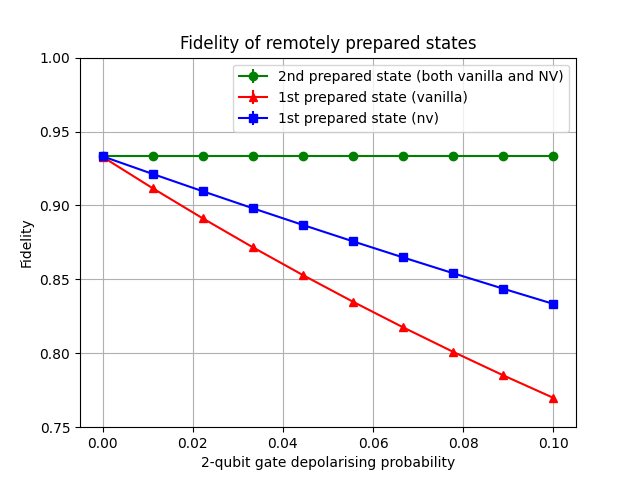
\includegraphics[scale=0.8]{figures/netqasm/plots/bqc_sweep_gate_noise_epr_fidelity.png}
  \caption{ Fidelity of the two remotely prepared states on the server in
        the BQC application. To remotely prepare a state, the client and server
        first create an EPR pair, and the client then measures its half in a
        specific basis while the server keeps its half stored in the
        communication qubit. This first prepared state is then moved to a memory
        qubit to free up the communication qubit for preparing the second state.
        This move operation has a negative effect on the fidelity of the first
        prepared state. Since the fidelity of the second prepared state only
        depends on the link entanglement generation, there is no difference
        between using vanilla or NV instructions. The values are from the same
        simulation experiment as for ~\cref{netqasm:fig:plot_bqc}. Error bars are
        negligible.}
  \label{netqasm:fig:plot_bqc_fidelity}
\end{figure}

\subsection{Relation to other results}
We note that a similar question of how many physical details to expose from lower-level layers (in our case the \ac{QNPU}) to higher-level layers (in our case the \ac{CNPU}) has also been evaluated in~\cite{murali2019fullstack}.
Their conclusion is that exposing and leveraging some of these details can indeed improve certain program success metrics.
That result agrees with that of ours, which shows that program execution quality can improve by exposing and leveraging unit modules and platform-specific \ac{NetQASM} flavors.


\section{Simulation details}
\label{netqasm:sec:simulation}

In this section we detail how simulations in \cref{netqasm:sec:evaluation} were
performed and what models and parameters were used. All simulations used the
\ac{NetQASM} SDK~\cite{git_netqasm}, using
NetSquid~\cite{netsquid,coopmans2021netsquid} as the underlying simulator. All
code used in these simulations can also be found at~\cite{git_squidasm}.


\subsection{Noise model}
In both the teleportation and the blind quantum computing scenario we used the
same model for nitrogen-vacancy centres in diamonds as was used
in~\cite{dahlberg2019linklayer} and~\cite{coopmans2021netsquid}. All gates
specified by the application in the SDK were translated to NV-specific gates,
see \cref{tab:gates}, using a simple compiler without any optimization. The
parameters used in the model from~\cite{dahlberg2019linklayer} are listed in
\cref{tab:gates,tab:noise}, together with an explanation and a reference.
\nq{ec_controlled_dir_xy} are the native two-qubit gates of the NV-platform,
ideally performing one of the unitary operations
\begin{align}
  U_\mathrm{ec_x}(\alpha) & = \begin{pmatrix}R_x(\alpha) & 0 \\ 0 & R_x(-\alpha) \end{pmatrix} \label{eq:crot_x} \\
  U_\mathrm{ec_y}(\alpha) & = \begin{pmatrix}R_y(\alpha) & 0 \\ 0 & R_y(-\alpha) \end{pmatrix} \label{eq:crot_y} \\
\end{align}
where $R_x(\alpha)$ and $R_y(\alpha)$ are the rotation matrices around $X$ and
$Y$, respectively. When sweeping the duration and noise of this two-qubit gate
the same value is also used for the \nq{carbon_xy_rot} ($X$- and $Y$-rotations
on the carbon) on the storage qubits, since these are also effectively done with
a similar operation also involving the communication qubit (electron). All noise
indicated by a fidelity in \cref{tab:noise} are applied as depolarising noise by
applying the perfect operation, producing the state $\rho_\mathrm{ideal}$, and
mapping this to
\begin{equation}\label{eq:depolarising}
  \rho_\mathrm{noisy}=(1-p)\rho_\mathrm{ideal} + \frac{p}{3}X\rho_\mathrm{ideal}X + \frac{p}{3}Y\rho_\mathrm{ideal}Y + \frac{p}{3}Z\rho_\mathrm{ideal}Z
\end{equation}
where $X$, $Y$ and $Z$ are the Pauli operators in
\cref{neqtasm:eq:pauli_x,netqasm:eq:pauli_y,netqasm:eq:pauli_z}, $p=\frac{4}{3}(1 - F)$, with $F$ being
the value specific in \cref{tab:noise}. Decoherence noise is specific as $T_1$
(energy/thermal relaxation time) and $T_2$ (dephasing time)~\cite{Nielsen2010}.

\begin{table}
  \centering
  \begin{tabular}{|c|c|c|}
    \hline
    Gate                      & Durations (ns) & Explanation                                                \\
    \hline\hline
    \texttt{electron\_init}        & 2e3            & Initialize a comm. qubit (electron) to $|0\rangle$ \\
    \texttt{electron\_rot}         & 5              & single-qubit rotation on comm. qubit (electron)    \\
    \texttt{measure}              & 3.7e3          & Measure communication qubit (electron)                     \\
    \texttt{carbon\_init}          & 3.1e5          & Initialize a storage qubit (carbon) to $|0\rangle$         \\
    \texttt{carbon\_xy\_rot}        & $t$            & $X$/$Y$-rotation on storage qubit (carbon)                 \\
    \texttt{carbon\_z\_rot}         & 5              & $Z$-rotation on storage qubit (carbon)                     \\
    \texttt{ec\_controlled\_dir\_xy} & $t$            & Native two-qubit gates, (\cref{eq:crot_x,eq:crot_y})     \\
    \hline
  \end{tabular}
  \caption{
    Gate durations for scenario \textbf{B} of \cref{netqasm:sec:evaluation}.
    $t$ is the value being swept in \cref{netqasm:fig:sweep_gate_time}.
    All values are from~\cite{dahlberg2019linklayer}.}
  \label{tab:gates}
\end{table}

\begin{table}
  \centering
  \begin{tabular}{||c|c|c|c||}
    \hline
    Parameter                 & Value        & Explanation                                                 \\
    \hline\hline
    \texttt{electron\_T1}          & 1 hour       & $T_1$ of communication qubit (electron)                     \\
    \texttt{electron\_T2}          & 1.46 seconds & $T_2$ of communication qubit (electron)                     \\
    \texttt{electron\_init}        & 0.99)        & Fidelity to initialize comm. qubit (electron)       \\
    \texttt{electron\_rot}         & 1.0          & Fidelity for $Z$-rotation on comm. qubit (electron) \\
    \texttt{carbon\_T1}            & 10 hours     & $T_1$ of storage qubit (carbon)                             \\
    \texttt{carbon\_T2}            & 1 second     & $T_2$ of storage qubit (carbon)                             \\
    \texttt{carbon\_init}          & 0.997        & Fidelity to initialize storage qubit (carbon)               \\
    \texttt{carbon\_z\_rot}         & 0.999        & Fidelity for $Z$-rotation on storage qubit (carbon)         \\
    \texttt{carbon\_xy\_rot}        & $f$          & Fidelity for $X$/$Y$-rotation on storage qubit (carbon)     \\
    \texttt{ec\_controlled\_dir\_xy} & $f$          & Fidelity for native two-qubit gate                          \\
    \texttt{prob\_error\_meas\_0}    & 0.05         & Probability of flipped measurement outcome for $|0\rangle$  \\
    \texttt{prob\_error\_meas\_1}    & 0.005        & Probability of flipped measurement outcome for $|1\rangle$  \\
    \texttt{link\_fidelity}        & 0.9          & Fidelity of generated entangled pair.                       \\
    \hline
  \end{tabular}
  \caption{
    Noise parameters for used in the simulations of \cref{netqasm:sec:evaluation}.
    $f$ is the value being swept in \cref{netqasm:fig:sweep_gate_noise} and \cref{netqasm:fig:plot_bqc}.
    All fidelities are realized by a applying depolarising noise as in \cref{eq:depolarising}.
    All values are from~\cite{coopmans2021netsquid}, except \nq{link_fidelity} which is set to relatively high value to avoid this being the major noise-contribution and preventing any conclusions to be made.
  }
  \label{tab:noise}
\end{table}

\subsection{BQC application and flavors}
In \cref{design_decisions_flavors} we simulated the blind quantum computation
(BQC) application from \cref{netqasm:fig:bqc_app}. The code for this is available at
\cite{git_squidasm}.

In the scenario when the application code was compiled to subroutines with the
vanilla lavour, the \ac{QNPU} had to map the vanilla instructions to NV-native
operations on the fly. We used the gate mappings listed below. For
convenience we use \nq{PI} and \nq{PI_OVER_2} for $\pi$ and $\frac{\pi}{2}$
respectively.

A \nq{h} (Hadamard) vanilla instruction was mapped to the following NV instruction sequence:
\begin{nqcode}
  rot_y PI_OVER_2
  rot_x PI\end{nqcode}

A \nq{cnot C S} vanilla instruction between a communication qubit (C) and a storage
qubit (S) (as specified in the unit module) was mapped to the following NV
instruction sequence:
\begin{nqcode}
  cx_dir C S PI_OVER_2
  rot_z C -PI_OVER_2
  rot_x S -PI_OVER_2\end{nqcode}

A \nq{cnot S C} vanilla instruction between a store qubit (S) and a communication
qubit (C) (as specified in the unit module) was mapped to the following NV
instruction sequence:
\begin{nqcode}
  rot_y C PI_OVER_2
  rot_x C PI
  rot_y S PI_OVER_2
  cx_dir C S PI_OVER_2
  rot_z C -PI_OVER_2
  rot_x S -PI_OVER_2
  rot_y S PI_OVER_2
  rot_y C PI_OVER_2
  rot_x C PI\end{nqcode}

A \nq{cphase C S} vanilla instruction between a communication qubit (C) and a storage
qubit (S) (as specified in the unit module) was mapped to the following NV
instruction sequence:
\begin{nqcode}
  rot_y S PI_OVER_2
  cx_dir C S PI_OVER_2
  rot_z C -PI_OVER_2
  rot_x S -PI_OVER_2
  rot_y S -PI_OVER_2\end{nqcode}
\section{Conclusion}
\label{sec:conclusion}
\ac{NetQASM} enables the development of quantum internet applications in a platform-independent manner.
It solves the question of dealing with the complexity of having both classical and quantum operations in a single program, while at the same time providing a relatively simple format for \ac{QNPU}-like layers to handle.
Multiple applications, such as remote teleportation and blind quantum computation, have already been implemented.
A simple compiler has been implemented that can translate code written in the higher-level SDK into \ac{NetQASM}.

Additionally to the work in this paper, we are also developing a physical implementation of the \ac{QNPU}.
\todo{Rewrite this part now that QNodeOS is finished}
One key component in this implementation is the \emph{Quantum Node Operating System} (QNodeOS), which acts as the bridge between the applications and the physical layer.
QNodeOS will be presented in a dedicated paper including results of a first integration test between \ac{NetQASM}, QNodeOS and underlying physical quantum hardware.
This will mark the first time a quantum network node has been programmed using platform-independent code.
\fi

\section{Data availability}
The data that support the findings of this study are openly available at the following DOI:
\url{https://doi.org/10.4121/21355329}.
The software packages created for this work (and used for the simulation) are
\url{https://github.com/QuTech-Delft/netqasm} (NetQASM) and \url{https://github.com/QuTech-Delft/squidasm} (SquidASM).
These packages are also part of the Quantum Network Explorer (QNE) SDK found at \url{https://quantum-network.com}.

\begin{xstretch}
\printbibliography[heading=subbibintoc,title={References},notcategory=noprint]
\end{xstretch}
